

%L'apparato sperimentale attualmente in uso ai LNS-INFN nell'ambito della Fase~2 del progetto NUMEN, costituito principalmente dallo spettrometro MAGNEX e dal Ciclotrone Superconduttore K800, viene brevemente illustrato nella prima parte di questo capitolo.
L'apparato sperimentale attualmente in uso ai LNS-INFN nell'ambito della Fase~2 del progetto NUMEN è costituito principalmente dallo spettrometro MAGNEX e dal Ciclotrone Superconduttore (CS).
Poiché la descrizione di tale apparato non costituisce l'argomento primario di questo lavoro di tesi, nella parte iniziale del capitolo vengono discusse soltanto le sue caratteristiche principali, rimandando alla vasta letteratura sul tema per informazioni più dettagliate (ad esempio~\cite{cavallaro:epja12, carbone:epja12, cappuzzello:epja16, cunsolo:epjst07}).

%Nella prima parte di questo capitolo vengono illustrate le principali caratteristiche dell'apparato sperimentale attualmente in uso ai LNS-INFN nell'ambito della Fase~2 del progetto NUMEN.
%Nella seconda parte viene descritta la configurazione dell'apparato adottata in occasione del test sui telescopi SiC-CsI svolto ad Aprile 2019, sottolineando le differenze rispetto a quella consueta.
Nell'ottica della Fase~4, l'intero apparato sperimentale subirà un importante upgrade, che, in particolare, modificherà radicalmente l'attuale sistema di rivelazione.
Nella seconda parte del capitolo viene, dunque, illustrato il progetto del nuovo Focal Plane Detector (FPD), soffermandosi sulla descrizione dei rivelatori che costituiranno i telescopi SiC-CsI del futuro muro dedicato alla~PID.

%Infine, nella terza parte vengono descritti i due prototipi di telescopio SiC-CsI, su cui ad Aprile~2019 è stato svolto un importante test al fine di verificare

Infine, nella terza parte vengono presentate le condizioni sperimentali in cui è stato svolto il test beam di Aprile~2019, il quale aveva l'obiettivo di valutare le prestazioni dei primi due prototipi di telescopio SiC-CsI e contestualmente verificare la risposta del primo esemplare di elettronica di front-end per il progetto NUMEN.

%del test sui telescopi SiC-CsI svolto ad Aprile~2019, esponendone le motivazioni, descrivendo la configurazione dell'apparato adottata e sottolineandone le differenze rispetto a quella consueta.

%\vspace{0.5 cm}

\section{\iflanguage{italian}{Lo spettrometro magnetico MAGNEX}{MAGNEX magnetic spectrometer}}

Lo spettrometro magnetico MAGNEX è un dispositivo ottico a grande accettanza, costituito da un quadrupolo per la focalizzazione sull'asse verticale, seguito da un dipolo per la dispersione sul piano orizzontale.
Grazie alle sue peculiarità,  MAGNEX riesce ad offrire, in un angolo solido molto grande e in un ampio range energetico, un'ottima risoluzione in energia, angolo e massa.
Ciò lo rende uno strumento ideale per l'analisi di eventi caratterizzati da sezioni d'urto molto basse, come è già stato dimostrato in~\cite{cappuzzello:epja16,pereira:plb12,oliveira:jpg13}.
Inoltre, esso consente di effettuare misure fino a zero gradi, comprendendo, dunque, la regione angolare di massimo interesse per lo studio del DCE.
In Figura~\ref{fig:magnex} è mostrata una foto dello spettrometro, in cui è possibile notare, andando da sinistra verso destra, la camera di scattering, il quadrupolo, il dipolo e il~FPD.


\begin{figure} [!t]
	\centering
	\includegraphics[width=\textwidth, keepaspectratio]{Grafici/magnex_etichette.png}
	\caption{Lo spettrometro magnetico MAGNEX.} \label{fig:magnex}
\end{figure}


La caratteristica che rende MAGNEX uno strumento unico è l'implementazione di una innovativa tecnica di ricostruzione delle traiettorie degli ioni, che consente di correggere le inevitabili aberrazioni originate dalla grande accettanza del dispositivo.
Dunque, a differenza di altri spettrometri magnetici, per MAGNEX è importante determinare non soltanto il punto di impatto sul piano focale ma anche la traiettoria completa. Ciò significa che è necessario misurare quattro parametri: una coppia, chiamata $(x_{foc}, y_{foc})$, individua il punto di impatto sul piano focale, l'altra, indicata con $(\theta_{foc}, \phi_{foc})$, si riferisce rispettivamente all'angolo orizzontale e a quello verticale della traccia al piano focale.
%Nel paragrafo successivo verrà esplicato in che modo vengono misurati tali parametri.
Il modo in cui tali grandezze vengono misurate sarà esplicato nel paragrafo successivo.
%Fra i quattro parametri al piano focale e i 
%
%
%Noti i quattro parametri al piano focale, si procede all'inversione dell'operatore $G$ che esprime il legame fra questi e i quattro parametri sul target.
%Se l'operatore $G^{-1}$ esiste, 
%
Noti i quattro parametri al piano focale, essi vengono utilizzati per risolvere le equazioni del moto di ogni singolo ione e da queste si ricavano i valori delle sezioni d'urto e delle altre quantità di interesse. 




%\clearpage 

%\vspace{0.5 cm}

\subsection{\iflanguage{italian}{L'attuale rivelatore di piano focale}{The present Focal Plane Detector}} \label{sez:fpd}

\begin{figure} [!p]
	\centering
	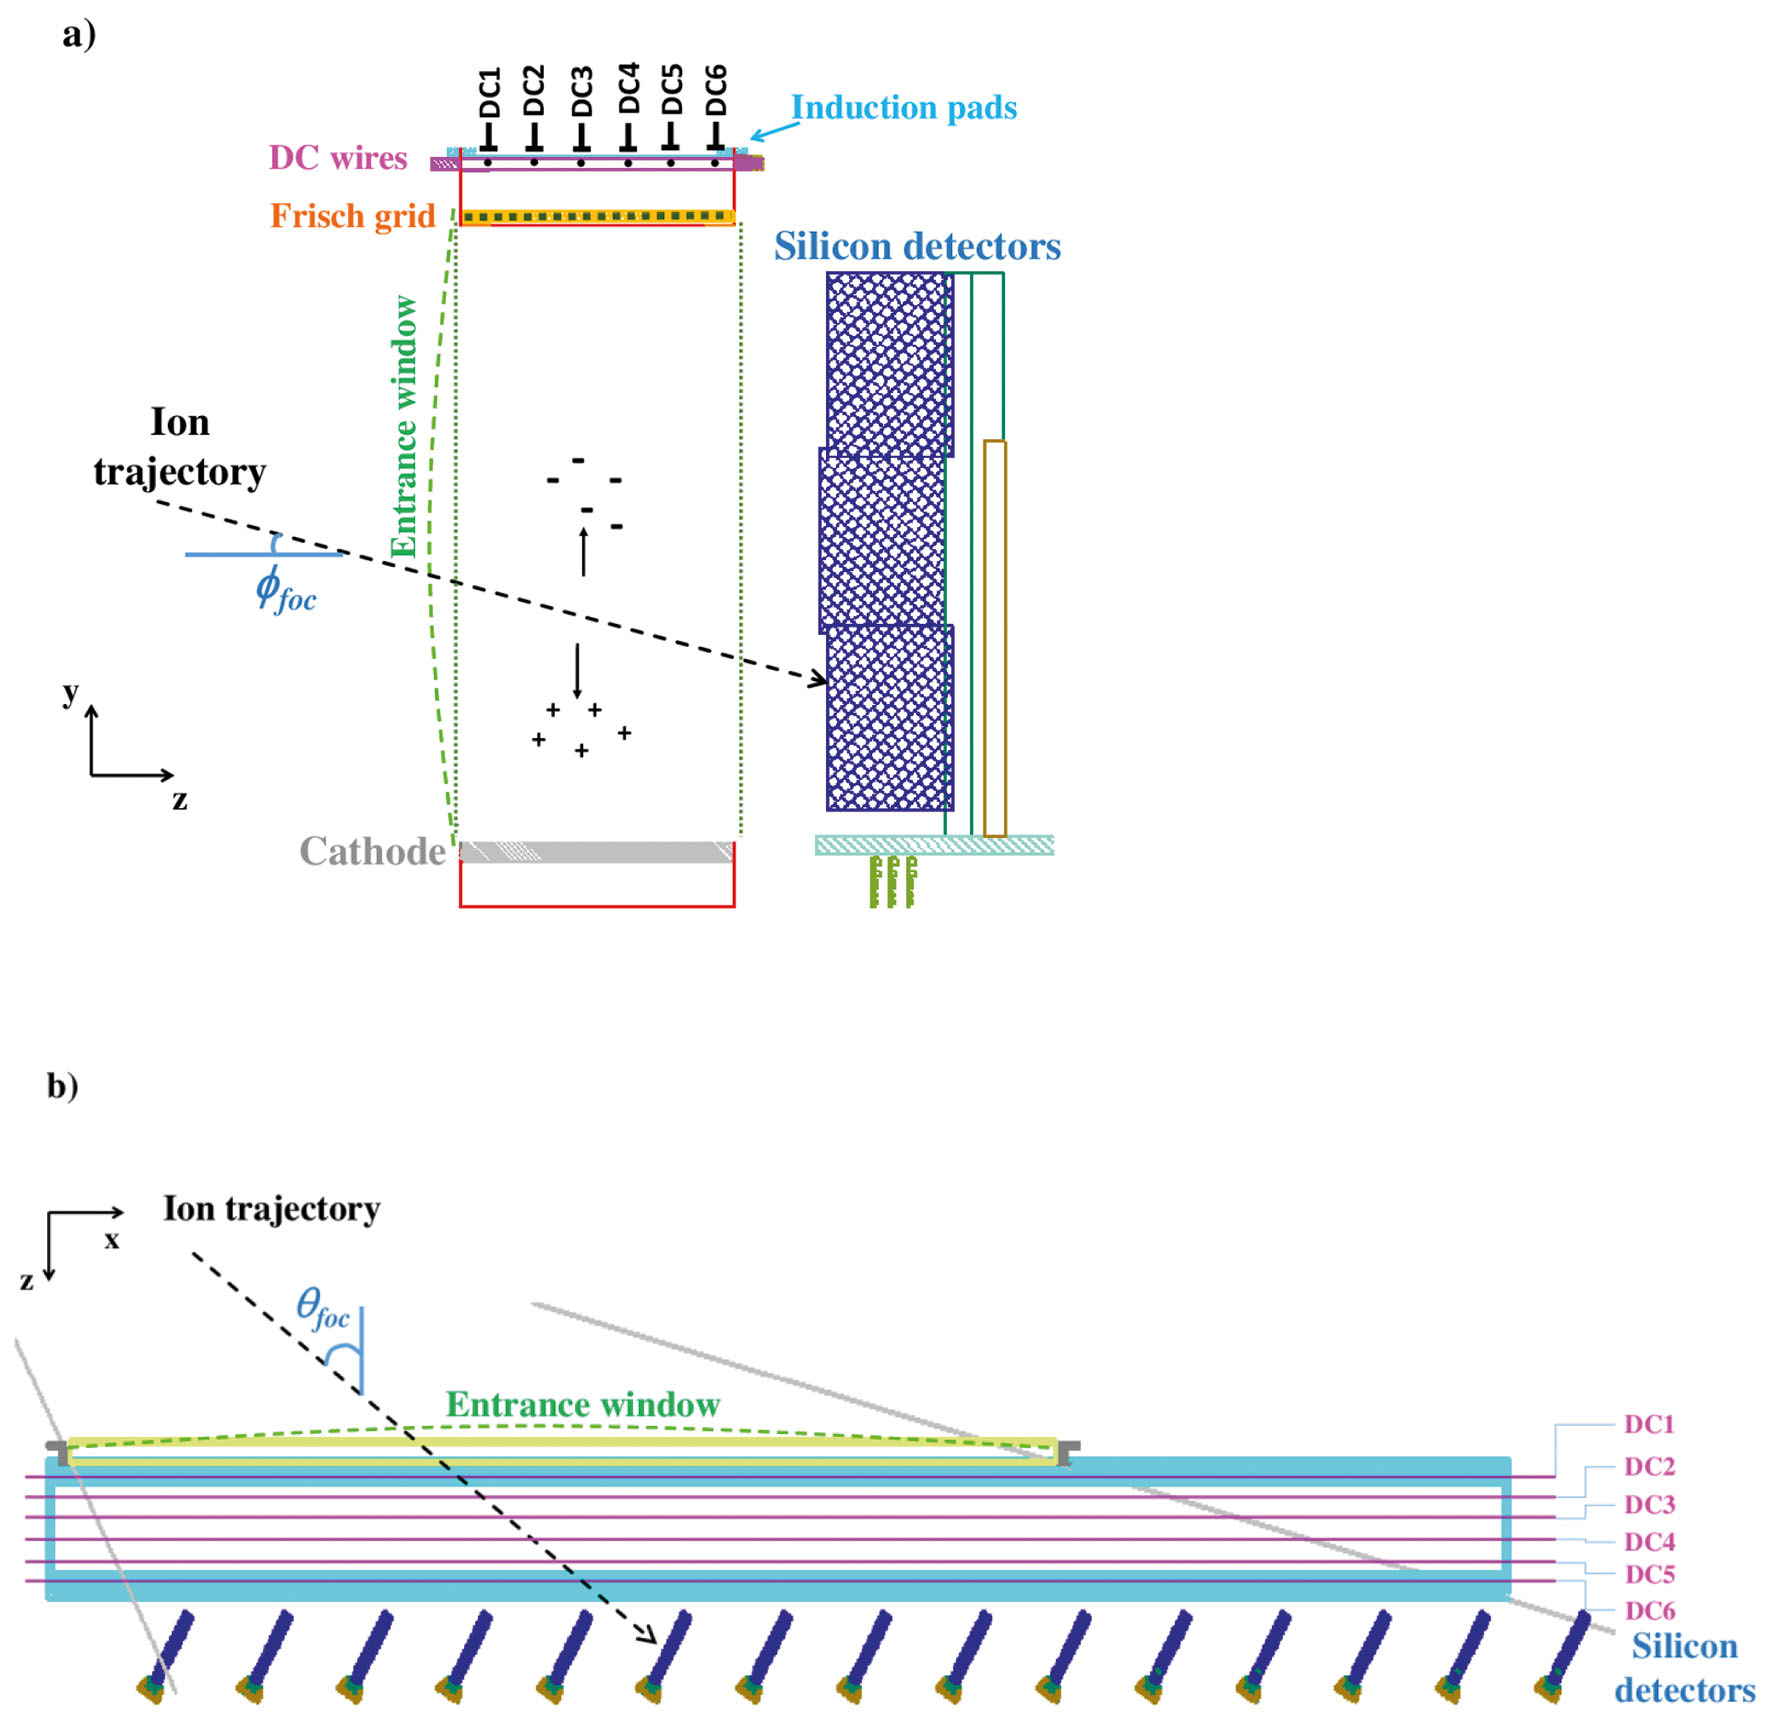
\includegraphics[width=\textwidth, keepaspectratio]{Grafici/fpd.png}
	\caption{Rappresentazione schematica del FPD: a) vista laterale; b) vista dall'alto. Figura tratta da~\cite{cappuzzello:epja18}.} \label{fig:fpd}
\end{figure}


L'attuale FPD di MAGNEX, la cui rappresentazione schematica è riportata in Figura~\ref{fig:fpd}, è un sistema di rivelazione ibrido, costituito da un tracciatore a gas a bassa pressione e da un muro di rivelatori al silicio.
Esso è posizionato a 1.91~m dall'uscita del dipolo e, al fine di minimizzare gli effetti dovuti alle aberrazioni cromatiche~\cite{cunsolo:nima01}, è inclinato di 59.2\textdegree{} rispetto ad un piano perpendicolare all'asse ottico.
%Una finestra di mylar spessa 1.5~$\mu$m è utilizzata per contenere il gas, solitamente costituito da N35 isobutano, segnando l'ingresso nel volume attivo.
L'ingresso nel volume attivo è definito da una finestra di Mylar spessa 2.5~$\mu$m, la quale è utilizzata per contenere il gas, solitamente costituito da N35 isobutano (C\ped{4}H\ped{10}) a pressioni di poche decine di~mbar.



%Il tracciatore a gas è formato da un sistema di sei fili al tungsteno placcati in oro, posti al di sotto di un anodo segmentato in pad. 
%Il tracciatore a gas lavora secondo il principio tipico delle camera a deriva.
%Il tracciatore a gas è essenzialmente una camera a deriva, in cui un sistema misto di fili e pad consente la misura dei quattro parametri necessari.
%Il tracciatore a gas, che consente la ricostruzione tridimensionale della traiettoria degli ioni, è formato da sei fili al tungsteno, indicati con DC\ped{\textit{i}}, e da un anodo segmentato in pad. 
%Al di sopra di ciascun filo si trova una fila di 224 pad
%Il tracciatore a gas è essenzialmente una camera a deriva, in cui un sistema costituito da sei fili (DC\ped{\textit{i}}) e da un anodo segmentato in pad consente la misura dei quattro parametri necessari per la ricostruzione tridimensionale della traccia.
%In particolare, al di sopra di ciascun filo è presente una fila di pad, le quali sono orientate parallelamente all'asse ottico.
Il tracciatore a gas, che consente la ricostruzione tridimensionale della traiettoria degli ioni, è formato da sei fili proporzionali (DC\ped{\textit{i}}) e da un anodo segmentato in sei file di pad, disposte in maniera che sopra ogni filo ci sia una fila di pad.
%Come descritto più avanti, i fili, sfruttando il principio di lavoro delle camere a deriva, danno una misura di sei posizioni verticali ($Y_i$), mentre le pad permettono di determinare sei posizioni orizzontali ($X_i$).
%Una griglia di Frisch è posta al di sotto dei fili, in quanto questi vengono anche utilizzati per misurare l'energia persa dagli ioni nel gas.
%Dal momento che i fili vengono anche utilizzati per misurare l'energia persa dagli ioni nel gas, una griglia di Frisch è posta al di sotto di essi, in modo da rendere il segnale indipendente dalla posizione dell'evento di ionizzazione.




Il muro di rivelatori al silicio, posto all'uscita del tracciatore, è formato da 60 rivelatori, organizzati in 20 colonne da 3 elementi ciascuna. 
%Ogni rivelatore, che ha un'area attiva di $70 \times 50$~mm\ap{2} ed uno spessore di 500~$\mu$m, è montato perpendicolarmente all'asse ottico.
Ogni rivelatore ha un'area attiva di $70 \times 50$~mm\ap{2} ed uno spessore di 500~$\mu$m.
%Ogni pad ha un'area attiva di $70 \times 50$~mm\ap{2} ed è spessa 500~$\mu$m, sufficienti per fermare i prodotti di reazioni nel range energetico di interesse. 
Essi vengono utilizzati per fermare gli ioni, misurandone l'energia residua e producendo il segnale di trigger per l'acquisizione. 

Quando una particella carica, attraversando la finestra di Mylar, entra nel volume attivo, perde energia nel gas producendo coppie elettrone-ione, le quali, sotto l'effetto di un campo elettrico uniforme, migrano rispettivamente verso la griglia di Frisch e il catodo. 
%mentre gli elettroni diffondono verso la griglia di Frisch, con una velocità che per questi ultimi è di circa $3 - 5 $~cm/$\mu$s. 
%La presenza di un campo elettrico costante provoca 
%La velocità di deriva tipica degli elettroni è di $3 - 5 $~cm/$\mu$s
Dopo aver attraversato la griglia, gli elettroni giungono in prossimità dei fili DC\ped{\textit{i}}, dove, a causa dell'elevato campo elettrico, danno luogo alla moltiplicazione a valanga. 
%La carica prodotta, proporzionale all'energia persa dalla particella nel gas, induce sulle pad una distribuzione di carica, della quale si calcola il baricentro. Questa operazione avviene per le sei file di pad, in modo tale che ai sei baricentri corrispondono sei misure di posizioni orizzantali $X_i$.
Alle tensioni e pressioni utilizzate, la carica secondaria prodotta genera un segnale proporzionale all'energia persa dalla particella nel gas. 
Poiché ciò avviene per ciascuno dei sei fili, si hanno sei segnali di perdita di energia, indicati con~$\Delta E_i$.





La stessa valanga induce sulle pad una distribuzione di carica, di cui si calcola il centro di gravità. Anche in questo caso l'operazione si ripete per le sei file di pad, così che vengono estratte sei misure di posizioni orizzontali~$X_i$.
A questo punto, effettuando un fit lineare sulle sei posizioni~$X_i$, si ottengono $x_{foc}$ e $\theta_{foc}$ rispettivamente dall'intercetta e dal coefficiente angolare della retta.

Superata la regione del tracciatore, la particella carica arriva al muro dei rivelatori al silicio, dove si ferma producendo un segnale proporzionale alla sua energia residua~$E_{resid}$. 
Lo stesso segnale viene utilizzato per calcolare l'intervallo di tempo impiegato dagli elettroni primari prodotti nel gas per raggiungere i fili DC\ped{\textit{i}}. 
%Dal momento che tale intervallo è proporzionale allo spazio percorso, si ottengono così sei misure di posizioni verticali~$Y_i$, dalle quali, grazie ad un fit lineare, si ricavano $y_{foc}$ e $\phi_{foc}$ in maniera analoga a quanto visto per $x_{foc}$ e $\theta_{foc}$.
Dal momento che la velocità di deriva è costante, tale intervallo di tempo è direttamente proporzionale allo spazio percorso. Si ottengono, dunque, sei misure di posizioni verticali~$Y_i$, dalle quali, grazie ad un fit lineare, si ricavano $y_{foc}$ e $\phi_{foc}$ in maniera analoga a quanto visto per $x_{foc}$ e $\theta_{foc}$.

È bene ricordare che, nelle camere a deriva a fili, la maggior parte del segnale è originata dal moto degli ioni positivi e non degli elettroni.
Di conseguenza, a causa della minore velocità degli ioni, tale tipologia di rivelatori può tipicamente sostenere rate dell'ordine di pochi~kHz. 
Questo aspetto, che costituisce una delle principali limitazioni all'intensità di fascio tollerabile dall'attuale FPD, deve essere superato nell'ottica della Fase~4. 
%Nasce da qui l'esigenza di sostituire l'attuale tracciatore con un sistema in grado di lavorare con un rate elevato di ioni pesanti. 
%Nasce da qui l'esigenza di sostituire l'attuale
Esso costituisce, dunque, uno dei principali motivi alla base del cambiamento del sistema di rivelazione degli eiettili con uno in grado di lavorare con un rate elevato di ioni pesanti. 
%Da qui trae origine la grande opera di cambiamento del sistema di rivelazione degli eiettili con uno in grado di lavorare con un rate elevato di ioni pesanti.

%\vspace{0.5 cm}

\section{\iflanguage{italian}{Il futuro rivelatore di piano focale}{Future Focal Plane Detector}}

%Il FPD previsto per la Fase~4 del progetto NUMEN manterrà una struttura simile a quella attuale, in quanto consisterà di un sistema di tracciamento tridimensionale a gas e di un muro di rivelatori per la PID.


%Il FPD previsto per la Fase~4 del progetto NUMEN consisterà di un tracciatore tridimensionale e di un muro di telescopi $\Delta E - E$.

Il FPD previsto per la Fase~4 del progetto NUMEN, pur mantenendo una struttura simile a quella attuale, dovrà fare uso di tecnologie innovative, molte delle quali sono ancora in fase di sviluppo.
Esso consisterà di un sistema di tracciamento tridimensionale a gas e di un muro di rivelatori per la~PID.


Il nuovo tracciatore, al momento in fase di sviluppo, dovrà garantire la misura ad alta risoluzione dei quattro parametri $ \left(  x_{foc}, y_{foc}, \theta_{foc}, \phi_{foc}  \right)$ necessari per la ricostruzione della traiettoria in condizioni di alti rate di particelle incidenti. 
%Esso sarà fondamentalmente costituito da tre parti: una regione di deriva per gli elettroni prodotti dalla ionizzazione, un elemento per la moltiplicazione degli elettroni e una scheda segmentata di readout.
Esso sarà fondamentalmente costituito da tre parti:
\begin{itemize}
	\item[--] una regione di deriva per gli elettroni prodotti dalla ionizzazione;
	\item[--] un elemento per la moltiplicazione degli elettroni, ovvero un Micro-Pattern Gas Detector (MPGD);
	\item[--] una scheda segmentata di readout.
\end{itemize}

Il suo principio di lavoro è il seguente: una particella carica incidente, dopo aver attraversato la finestra di mylar per il contenimento del gas, produce lungo la sua traiettoria una traccia di coppie elettrone-ione. 
%Il campo elettrico uniforme fra il catodo e l'elemento per la moltiplicazione guida gli elettroni
%Il campo elettrico uniforme fra catodo e anodo guida gli elettroni primari verso l'elemento di moltiplicazione
Sotto l'azione del campo elettrico uniforme presente fra catodo e anodo, gli elettroni primari si muovono con velocità costante nella regione di deriva fino a raggiungere il MPGD.
Analogamente a quanto visto nel Paragrafo~\ref{sez:fpd}, dalla misura del tempo di deriva degli elettroni primari è possibile estrarre l'informazione sulla posizione e sull'angolo verticali.
%Giunti al MPGD, gli elettroni primari danno origine ad una moltiplicazione a valanga, che risulta nella formazione di un jet elettronico. 
In seguito, gli elettroni primari giungono al MPGD, che dovrebbe essere basato sulla tecnologia delle M-THGEM.
Ciascun THGEM è costituito da una pila di fogli di materiale isolante (solitamente kapton) rivestiti su entrambe le facce con uno strato metallico.
I fogli, che possono avere superfici molto grandi, sono tra loro distanti pochi~mm e si trovano immersi nel gas.
Ogni foglio presenta una trama regolare di fori, i quali hanno un diametro di 0.6~mm.
%Una differenza di potenziale è applicata tra le due superfici metalliche, in modo che gli elettroni vengano guidati verso i fori, dove, incontrando un campo elettrico molto intenso, viene prodotta una moltiplicazione a valanga.
Quando gli elettroni arrivano al primo foglio, la differenza di potenziale applicata tra le due superfici metalliche li guida verso i fori, dove, sotto l'effetto di un campo elettrico molto intenso, producono una moltiplicazione a cascata.
A questo punto, la valanga viene indirizzata da un'ulteriore differenza di potenziale verso il foglio successivo, dando luogo ad una seconda moltiplicazione.
Il processo si ripete per i diversi stadi (2 o 3 a seconda del sistema utilizzato) della M-THGEM, fino a raggiungere fattori di guadagno dell'ordine di $10^4 \div 10^5$. 
Superato l'ultimo foglio, la valanga viene guidata dal campo elettrico verso la scheda segmentata di readout, dove induce su delle strip un impulso di carica. 
Di conseguenza, note le strip coinvolte, è possibile misurare la posizione e l'angolo orizzontali. 





Dopo aver attraversato il tracciatore a gas, la particella carica raggiunge il muro per la PID.
%, che, come anticipato nel Paragrafo~\ref{sez:sistema_identif_part}, sarà costituito da una matrice di telescopi $\Delta E - E$ basati sulla tecnologia SiC-CsI.
%Poiché la simulazione svolta per questo lavoro di tesi verte principalmente su tale argomento,
Poiché l'argomento principale del presente lavoro di tesi consiste nella simulazione di tale sistema di identificazione, per maggiore chiarezza si è preferito discuterne le caratteristiche nella sezione successiva.

%La scelta della tecnologia da utilizzare per il MPGD è oggi orientata verso le Thick-GEM, che, grazie alla loro capacità di sostenere rate fino al MHz/mm\ap{2}, sono adatte agli scopi di NUMEN.
Grazie alla loro capacità di sostenere rate fino al MHz/mm\ap{2}, le M-THGEM costituiscono un'ottima soluzione alle esigenze di NUMEN anche per applicazioni a bassa pressione.
%Tuttavia, diverse delle condizioni in cui questo tipo di rivelatori è abitualmente impiegato non sono attuabili per NUMEN. 
%In primo luogo, le Thick-GEM sono tipicamente utilizzate con gas a pressione atmosferica, mentre il FPD opera solitamente a pressioni di alcune decine di mbar.
%Inoltre, esse spesso sono utilizzate per rivelare particelle in condizioni di Minimum Ionizing Particle, mentre gli ioni di interesse per NUMEN saranno ben lontani da tali energie.
%In aggiunta, dal momento che diversi tipi di ioni raggiungono il rivelatore, il tracciatore deve avere ...
%Dunque, sebbene incoraggianti risultati siano stati recentemente ottenuti~\cite{cortesi:rsi17}, questa soluzione richiede un'intensa attività di sviluppo.


\begin{figure} [!p]
	\centering
	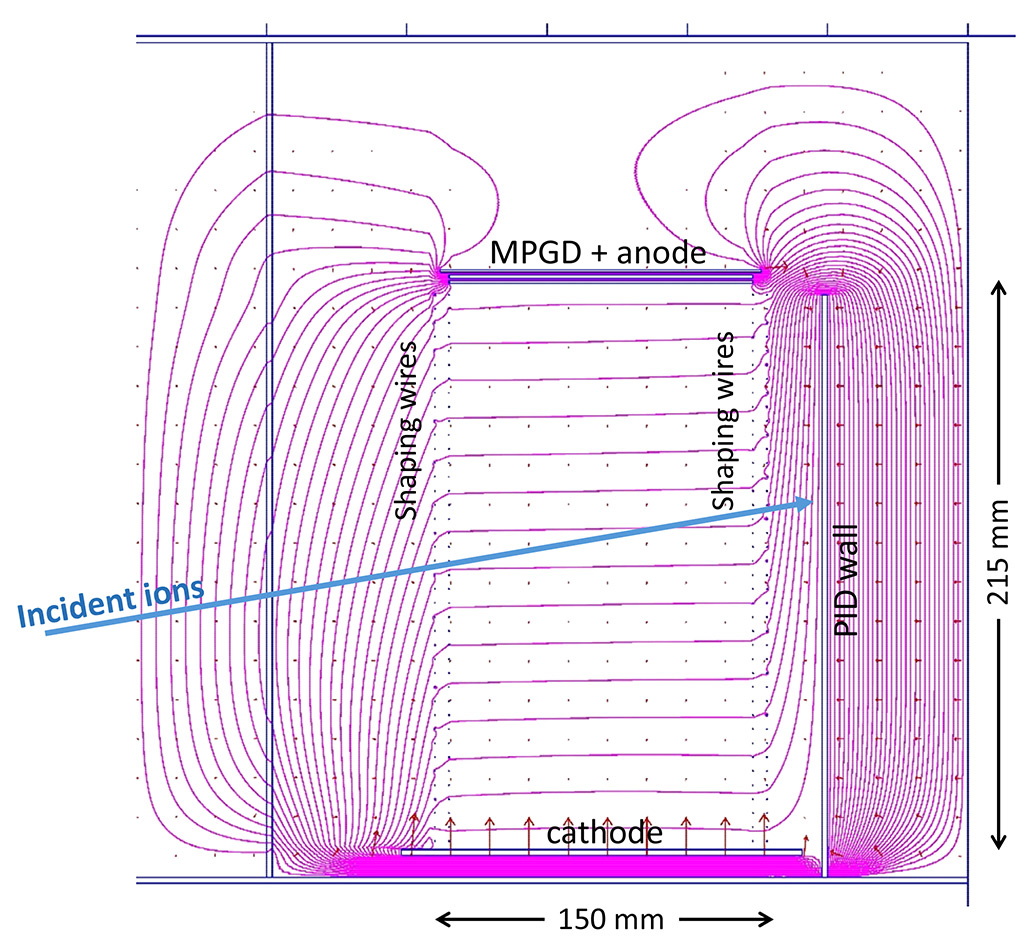
\includegraphics[scale=0.3]{Grafici/nuovo_fpd.png}
	\caption{Rappresentazione schematica del previsto FPD. Le linee magenta indicano le superfici equipotenziali, mentre le frecce mostrano il corrispondente campo elettrico. Figura tratta da~\cite{cappuzzello:epja18}.} \label{fig:nuovo_fpd}
\end{figure}


\begin{figure} [!p]
	\centering
	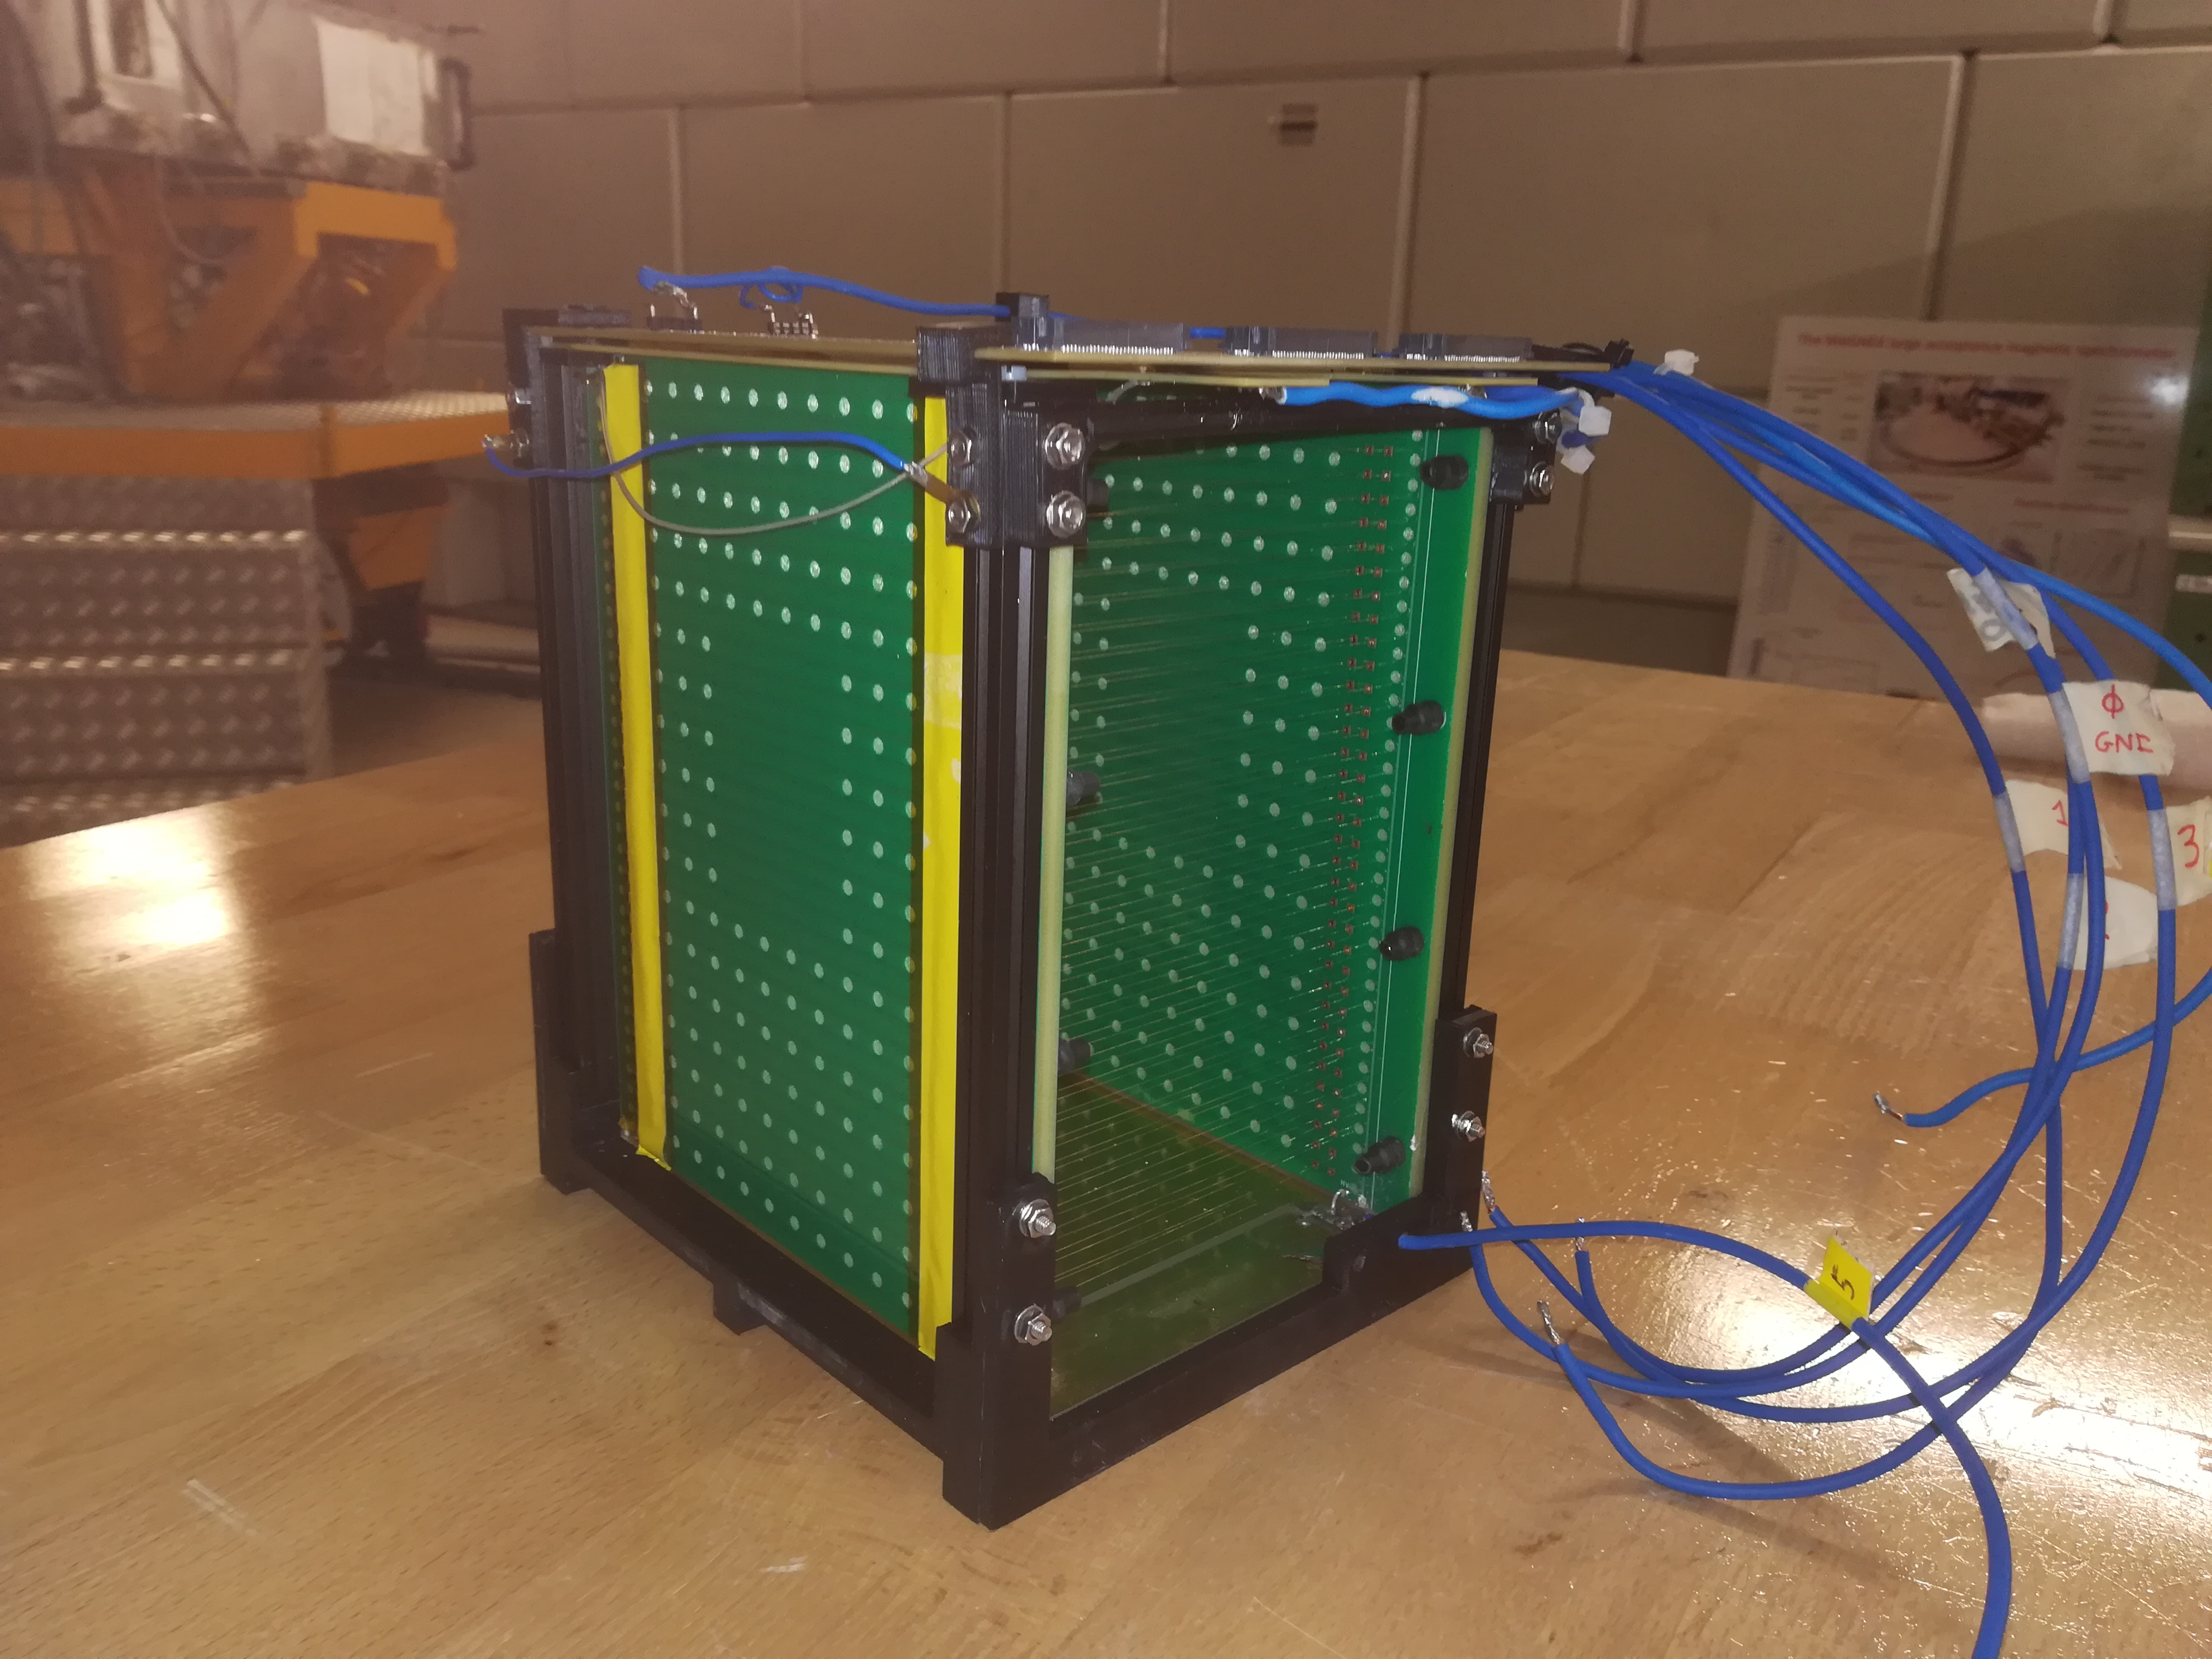
\includegraphics[width=\textwidth, keepaspectratio]{Grafici/castelletto3.jpg}
	\caption{Il prototipo del sistema di tracciamento previsto per NUMEN.} \label{fig:castelletto}
\end{figure}



Una rappresentazione schematica del futuro FPD è mostrata in Figura~\ref{fig:nuovo_fpd}, dove sono raffigurate anche le superfici equipotenziali calcolate con il codice Poisson-Superfish~\cite{superfish:87}: le linee quasi parallele indicano che nella regione di deriva il campo elettrico è piuttosto uniforme.


Un prototipo di dimensioni ridotte, mostrato in Figura~\ref{fig:castelletto}, è stato realizzato per individuare le migliori soluzioni in termini di geometria, tensioni applicate, MPGD ed elettronica.








%\vspace{0.3 cm}

%\clearpage
%\section{\iflanguage{italian}{Il test sui telescopi SiC-CsI}{Experimental setting for the test}}

\section{\iflanguage{italian}{I telescopi SiC-CsI}{SiC-CsI telescope detectors}}

%Ad Aprile 2019 è stato svolto un test sui primi due prototipi di telescopi SiC-CsI, allo scopo di confrontarne la risposta con il sistema attualmente utilizzato.
%Ad Aprile 2019 è stato svolto un test sui primi due prototipi di telescopi SiC-CsI, allo scopo di valutarne la risposta, confrontandola con quella del sistema attualmente utilizzato.


%Dopo aver realizzato 
%Per verificare se la risposta di un telescopio formato da uno stadio $\Delta E$ al SiC seguito da un cristallo di CsI poteva garantire prestazioni di identificazione degli ioni confrontabili con quelle accessibili con l'attuale apparato, è stato svolto un test per una durata complessiva di cinque giorni.
%Dal momento che tali rivelatori non sono ancora uno standard nel mondo della fisica ma rappresentano una tecnologia nuova, è stato svolto un test per verificare se le loro prestazioni possono soddisfare le esigenze di NUMEN.

%Come illustrato nel Paragrafo~\ref{sez:sistema_identif_part}, i rivelatori al SiC sono stati scelti nell'ambito del progetto per assolvere al ruolo di sistema di PID
%Sono stati, dunque, assemblati due telescopi SiC-CsI, di cui si è studiata la risposta in termini di PID.

%Come illustrato nel Paragrafo~\ref{sez:sistema_identif_part}, i rivelatori al SiC sono stati scelti nell'ambito del progetto per identificare i prodotti di reazione

%Quando si studiano le reazioni fra ioni pesanti, l'identificazione in numero atomico, massa e carica dei prodotti di reazione è una componente indispensabile che, a seconda delle esigenze, viene eseguita sfruttando vari metodi.
%Una delle tecniche più diffuse prevede l'utilizzo di telescopi $\Delta E - E$.
Quando si studiano le reazioni fra ioni pesanti, l'identificazione in numero atomico ($Z$), massa ($A$) e carica ($q$) dei prodotti di reazione è una componente indispensabile per la ricostruzione e la misura delle sezioni d'urto.
Il progetto NUMEN, a tale scopo, propone l'utilizzo combinato di diversi metodi: l'identificazione in $Z$ verrà svolta mediante la tecnica $\Delta E - E_{resid}$, mentre per quella in $A$ e $q$ si utilizzeranno anche la deflessione dovuta alla forza di Lorentz e il tempo di volo degli ioni.
%Come anticipato nel Paragrafo~\ref{sez:sistema_identif_part}, il progetto NUMEN ha individuato come possibile soluzione per la PID in condizioni di alti rate di particelle incidenti l'utilizzo di telescopi $\Delta E - E$, in cui il primo stadio è costituito da un rivelatore al carburo di silicio (SiC), mentre il secondo è uno scintillatore allo CsI.
In particolare, come anticipato nel Paragrafo~\ref{sez:sistema_identif_part}, i telescopi $\Delta E - E_{resid}$ saranno costituiti da un primo stadio basato su un rivelatore al carburo di silicio (SiC), seguito da uno scintillatore allo ioduro di cesio (CsI).
Il progetto al momento prevede la realizzazione di un muro composto da 1230 telescopi, arrangiati in 41 colonne.
Ogni colonna è, a sua volta, costituita da 3 moduli contenenti una matrice di $2 \times 5$ telescopi ciascuno.
In Figura~\ref{fig:muro_telescopi} è riportato uno schema di come dovrebbe apparire il futuro muro per la PID.

Prima di proseguire, vediamo più in dettaglio le principali caratteristiche dei rivelatori al SiC e degli scintillatori allo CsI, sottolineando gli aspetti che  hanno guidato verso la loro scelta nell'ambito di NUMEN.


\begin{figure} [!t]
	\centering
	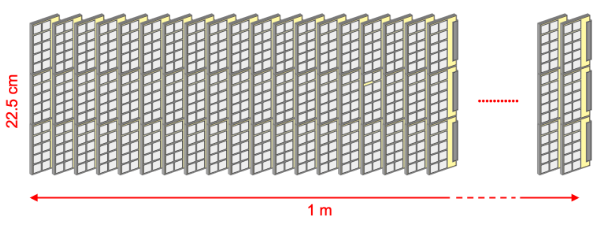
\includegraphics[width=\textwidth, keepaspectratio]{Grafici/muro_telescopi.png}
	\caption{Schema del muro di telescopi previsto per NUMEN.} \label{fig:muro_telescopi}
\end{figure}



%Il fascio utilizzato nel test era costituito da \ce{^{20}Ne}, mentre i bersagli erano \ce{^{197}Au} e \ce{^{12}C}




%\vspace{0.5 cm}
%\clearpage

%\subsection{\iflanguage{italian}{I telescopi SiC-CsI}{SiC-CsI telescope detectors}}

\subsection{\iflanguage{italian}{I rivelatori al carburo di silicio}{Silicon carbide detectors}}


%I dispositivi al SiC costituiscono oggi una promettente realtà nel campo dei rivelatori per la fisica, 
Grazie alle sue interessanti proprietà, il SiC costituisce oggi una promettente realtà nel campo della realizzazione di rivelatori per la fisica, configurandosi come una potenziale alternativa al silicio nelle applicazioni che richiedono una grande resistenza alle radiazioni.
%La larghezza della sua gap, quasi tripla rispetto a quella del silicio, se da un lato aumenta l'energia media per la produzione di una coppia elettrone-lacuna, dall'altro riduce il numero di portatori di carica generati per agitazione termica, mantenendo, dunque, un ottimo rapporto segnale-rumore.
%
%La larghezza della sua gap, quasi tripla rispetto a quella del silicio, se da un lato riduce il numero di portatori di carica generati per agitazione termica, dall'altro aumenta l'energia media per la produzione di una coppia elettrone-lacuna. 
%La larghezza della sua gap, essendo quasi tripla rispetto a quella del silicio, aumenta l'energia media per la produzione di una coppia elettrone-lacuna.
%Esso fa parte dei semiconduttori a grande larghezza di banda
%Dal momento che la larghezza della sua gap è quasi tripla rispetto a quella del silicio, l'energia media per la produzione di una coppia elettrone-lacuna nel SiC è maggiore di quella nel silicio. 
La caratteristica che ha suscitato grande interesse nella comunità scientifica nei confronti di questo materiale deriva dalla larghezza della sua gap, che risulta essere quasi tripla rispetto a quella del silicio.
Ciò implica diverse conseguenze: in primo luogo, dal momento che l'energia media per la produzione di una coppia elettrone-lacuna nel SiC è quasi tre volte quella nel silicio, a parità di energia una particella incidente su un rivelatore al SiC crea un terzo dei portatori di carica prodotti in un rivelatore al silicio.
Dunque, ne deriva un'inferiore ampiezza del segnale generato e, conseguentemente, un peggioramento della risoluzione, in quanto la componente statistica di tale grandezza è inversamente proporzionale alla radice quadrata del numero di portatori~\cite{knoll:10}.
%\textcolor{red}{???} Tuttavia, gli ioni pesanti di interesse per NUMEN, rilasciando molta energia nel rivelatore, producono un numero elevato di portatori, in modo tale che le fluttuazioni statistiche risultano trascurabili.
%
%% MODIFICHIAMO QUESTA PARTE
%Ciò significa che, a parità di energia, una particella incidente su un rivelatore al SiC crea un terzo dei portatori di carica prodotti in un rivelatore al silicio, generando, dunque, un segnale di ampiezza inferiore.
%Ciò significa che, a parità di energia, una particella incidente su un rivelatore al SiC crea un terzo dei portatori di carica prodotti in un rivelatore al silicio.
%
%% PRIMA DELLA CORREZIONE DEL PROF
%Dunque, a parità di energia, una particella incidente su un rivelatore al SiC crea un terzo dei portatori di carica prodotti in un rivelatore al silicio, generando, di conseguenza, un segnale di ampiezza inferiore.
%Ciò ha come conseguenza che il segnale generato presenta un'ampiezza inferiore.
%Ciò ha come effetto un peggioramento della risoluzione, in quanto la componente statistica di tale grandezza è inversamente proporzionale alla radice quadrata del numero di portatori~\cite{knoll:10}.
%Tuttavia, la maggiore larghezza della gap determina una riduzione del numero di coppie generate per agitazione termica, che risulta, dunque, in una diminuzione della corrente inversa e del livello di rumore.
%Tuttavia, la maggiore larghezza della gap determina l'estrema resistenza alle radiazioni del SiC, poiché, sebbene a causa del danno da radiazioni possano introdursi dei livelli in banda proibita, questi possono restare piuttosto lontani dalle bande di conduzione e di valenza.
%Di conseguenza, le transizioni elettroniche da o verso tali livelli possono risultare sfavorite, in modo da non causare un aumento significativo della corrente inversa.
%Tuttavia, la maggiore larghezza della gap determina l'estrema resistenza alle radiazioni del SiC.
%Ciò può essere spiegato nel modo seguente: l'irraggiamento può causare l'introduzione di livelli in banda proibita

%
%% ALTRIMENTI CI METTO QUESTO (Tratto da EPJ)
Tuttavia, la maggiore larghezza della gap del SiC, insieme all'elevata forza dei suoi legami chimici, determina la sua estrema resistenza alle radiazioni.
Tale proprietà può essere spiegata nel modo seguente: quando una particella carica attraversa un rivelatore, oltre a ionizzare ed eccitare gli atomi del mezzo, può causare la comparsa nel reticolo cristallino di interstizi, vacanze o strutture più complesse.
Questi difetti possono introdurre dei livelli nella banda proibita, che alterano le proprietà originali del semiconduttore; in particolare, i principali effetti macroscopici sono: l'aumento della corrente inversa, il cambiamento della tensione di svuotamento e la riduzione dell'efficienza di raccolta di carica, in quanto i difetti agiscono come trappole per i portatori di carica.
Dal momento che il SiC ha una gap piuttosto grande, i livelli nella banda proibita possono comunque risultare piuttosto distanti dalle bande di valenza e di conduzione, in modo tale da sfavorirne il popolamento.
Di conseguenza, sebbene si verifichi la comparsa di tali livelli, la corrente inversa non subisce un aumento significativo.

Inoltre, bisogna ricordare che il danno causato da protoni, neutroni o particelle al MIP è totalmente diverso da quello prodotto da ioni pesanti; infatti, mentre i primi, depositando poca energia nel rivelatore, danno luogo principalmente a fenomeni di dislocamento di singoli atomi, i secondi, rilasciando elevate quantità di energia, possono originare lo spostamento di interi cluster.
Se la prima tipologia di danno può essere contrastata mantenendo i rivelatori a bassa temperatura (come avviene con il silicio), la seconda dipende soltanto dalla resistenza del reticolo.
%Inoltre, l'elevata forza dei legami chimici del SiC si traduce in un'energia di dislocamento di $30 \div 40$~eV, circa tre volte superiore a quella del silicio.
In entrambi i casi il SiC esibisce delle notevoli proprietà di robustezza, in quanto l'elevata forza dei suoi legami chimici si traduce in un'energia di dislocamento di $30 \div 40$~eV, circa tre volte superiore a quella del silicio. 




%Questo ha due diverse conseguenze sul segnale generato: in primis, ne diminuisce l'ampiezza; in secondo luogo, ne aumenta le fluttuazioni relative, in quanto la componente statistica della risoluzione è inversamente proporzionale alla radice quadrata del numero dei portatori~\cite{knoll:10}.
%Se il primo problema può essere risolto aumentando l'amplificazione del segnale, il secondo è intrinseco del rivelatore.
%, dando origine a due diversi problemi: in primo luogo, il segnale generato presenta un'ampiezza inferiore, 
%di conseguenza, 
%di conseguenza, non soltanto il segnale generato presenta un'ampiezza inferiore, ma la risoluzione energetica 
%Di conseguenza, dal momento che la componente statistica della risoluzione è inversamente proporzionale alla radice quadrata del numero dei portatori~\cite{knoll:10}, i rivelatori al SiC hanno una risoluzione  
%
%Dunque, i rivelatori al SiC generano segnali di ampiezza inferiore rispetto a quelli dei rivelatori al silicio.
%
%% CASSIAMO QUESTA PARTE
%Tuttavia, gli ioni pesanti di interesse per NUMEN dovrebbero generare un numero elevato di coppie elettrone-lacuna, così che l'ampiezza del segnale dovrebbe essere sufficientemente grande.
%
%
%Inoltre, i rivelatori al SiC hanno un ottimo rapporto segnale-rumore anche a temperature piuttosto alte, mentre i rivelatori al silicio hanno, in alcuni casi, bisogno di un sistema di raffreddamento.


%Oltre alla resistenza alle radiazioni, un ulteriore vantaggio rispetto ai rivelatori al silicio riguarda il comportamento a temperature piuttosto alte: mentre i rivelatori al SiC continuano ad avere un ottimo rapporto segnale-rumore, i rivelatori al silicio mostrano un aumento della corrente inversa, rendendo a volte necessario l'utilizzo di sistemi di raffreddamento.
Oltre alla resistenza alle radiazioni, i rivelatori al SiC presentano un ulteriore vantaggio rispetto a quelli al silicio: la maggiore larghezza della gap determina una riduzione del numero di coppie generate per agitazione termica, che risulta, dunque, in una diminuzione della corrente inversa e del livello di rumore.
Di conseguenza, anche a temperature piuttosto alte, i rivelatori al SiC continuano ad avere un ottimo rapporto segnale-rumore, mentre i rivelatori al silicio mostrano un aumento della corrente inversa, rendendo a volte necessario l'utilizzo di sistemi di raffreddamento.

Grazie ai notevoli progressi in campo tecnologico, oggi i rivelatori al SiC possono essere realizzati mediante una giunzione p-n, polarizzata inversamente per aumentare l'estensione della regione svuotata e per migliorare l'efficienza di raccolta dei portatori di carica.
Quando una particella carica attraversa il rivelatore, perde energia generando coppie elettrone-lacuna, le quali, in presenza di un campo elettrico, si muovono verso gli elettrodi, producendo un segnale elettrico proporzionale all'energia depositata.

Nella rivelazione di ioni pesanti ad energie maggiori di diverse decine di~MeV (come quelli di interesse per NUMEN), i rivelatori al SiC esibiscono risoluzioni energetiche confrontabili con quelle dei dispositivi al silicio, in quanto viene rilasciata molta energia nel rivelatore e, pertanto, viene prodotto un numero elevato di portatori di carica.
Dunque, le fluttuazioni statistiche sul segnale risultano piccole determinando un trascurabile effetto sulla risoluzione in energia, quest'ultima dominata da altri fattori come il rumore termico, l'accoppiamento con l'elettronica di front-end, etc.
%Inoltre, recenti test hanno dimostrato che con un rivelatore da 100~$\mu$m di spessore è possibile ottenere una risoluzione energetica dello 0.4\%~FWHM per le particelle $\alpha$ dell'\ce{^{241}Am} a 5486~keV~\cite{tudisco:sensors18}, mentre con i rivelatori al silicio per le stesse particelle si possono raggiungere valori dello 0.2\% FWHM~\cite{steinbauer:nimb94}.

Recentemente, diversi test sono stati condotti su rivelatori al SiC dello stesso tipo di quelli che verranno utilizzati per NUMEN: in uno di questi test sono state messe a confronto le prestazioni in termini di risoluzione energetica di tale rivelatore con quelle di un rivelatore al silicio~\cite{tudisco:sensors18}.
I risultati, riportati in Figura~\ref{fig:tudisco_spettro}, dimostrano che col rivelatore al SiC è possibile ottenere una risoluzione energetica dello 0.4\%~FWHM per le particelle $\alpha$ dell'\ce{^{241}Am} a 5486~keV, mentre col rivelatore al silicio per le stesse particelle si è raggiunto un valore dello 0.22\%~FWHM.
\begin{figure} [!p]
	\centering
	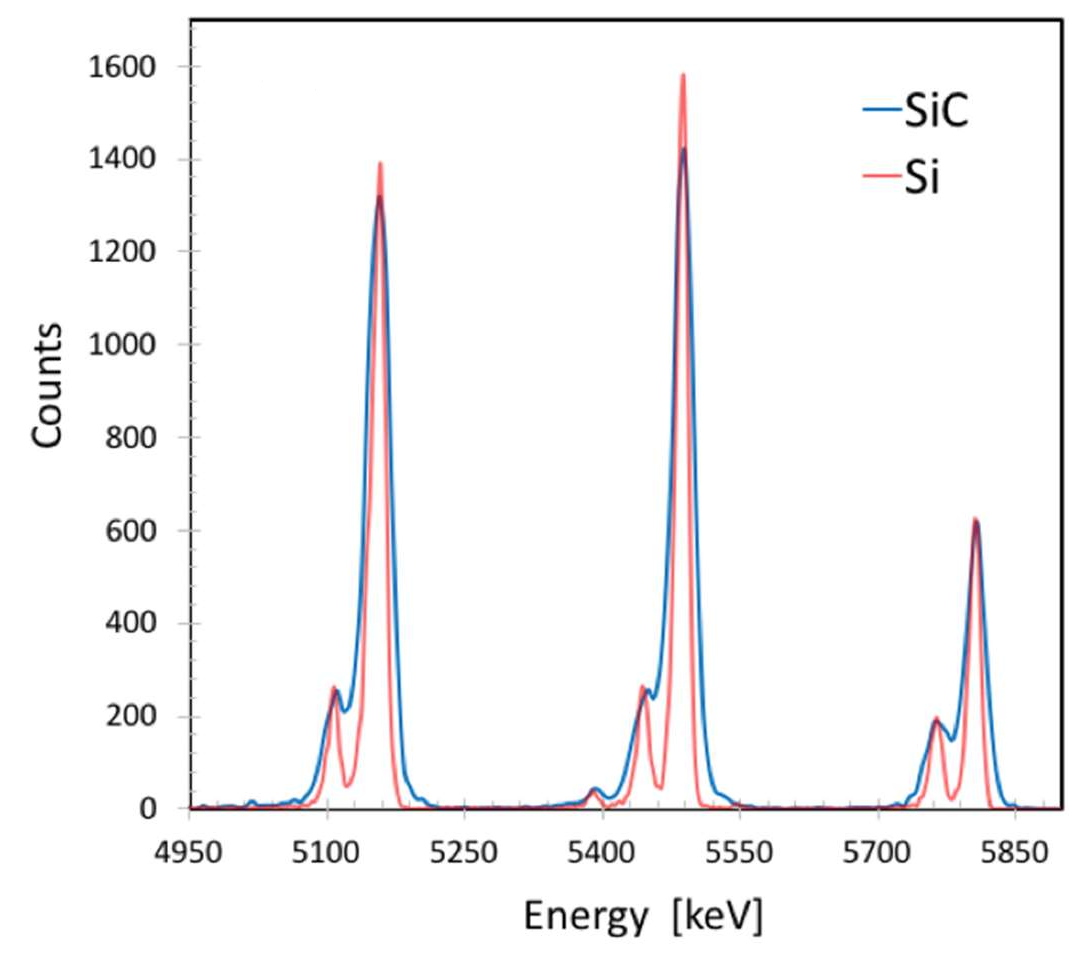
\includegraphics[width=\textwidth, keepaspectratio]{Grafici/spettro_sic_tagliato.png}
	\caption{Spettro energetico della sorgente $\alpha$ (\ce{^{239}Pu}, \ce{^{241}Am}, \ce{^{244}Cm}) misurato da un rivelatore al silicio Hamamatsu S3590 e da un rivelatore al SiC. Figura tratta da~\cite{tudisco:sensors18}.} \label{fig:tudisco_spettro}
\end{figure}
In un altro test~\cite{ciampi:nima19}, il rivelatore al SiC è stato adoperato per la realizzazione di un telescopio SiC-CsI, simile a quelli previsti per NUMEN.
Tale telescopio, la cui rappresentazione schematica è mostrata in Figura~\ref{fig:ciampi_telescopio}, è stato utilizzato per l'identificazione degli eiettili prodotti dalla collisione di un fascio di \ce{^{40}Ca} e \ce{^{48}Ca} a 40~AMeV con un bersaglio di \ce{^{12}C}. 
Le correlazioni $\Delta E - E_{resid}$ sono riportate in Figura~\ref{fig:ciampi_deltaE_E}: come si può notare, i differenti elementi sono ben identificati fino a $Z \sim 20$, consentendo perfino un'identificazione in $A$ per $Z \lesssim 3$.


\begin{figure} [!t]
	\centering
	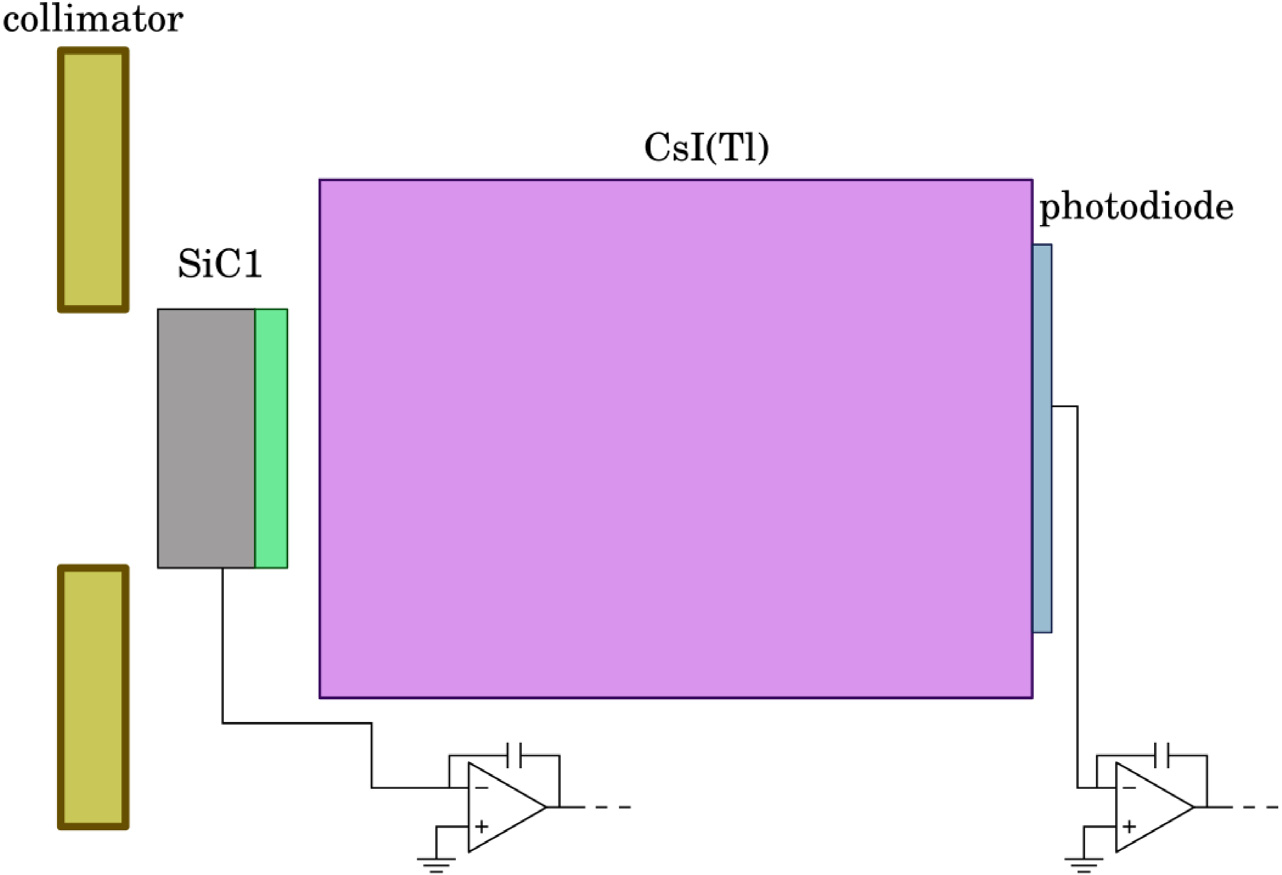
\includegraphics[scale=0.25]{Grafici/ciampi-telescopio.png}
	\caption{Rappresentazione schematica del telescopio SiC-Csi. Per il primo stadio, il substrato (grigio) e l'area sensibile (verde chiaro) sono mostrati in proporzione. Figura tratta da~\cite{ciampi:nima19}.} \label{fig:ciampi_telescopio}
\end{figure}



\begin{figure} [!p]
	\centering
	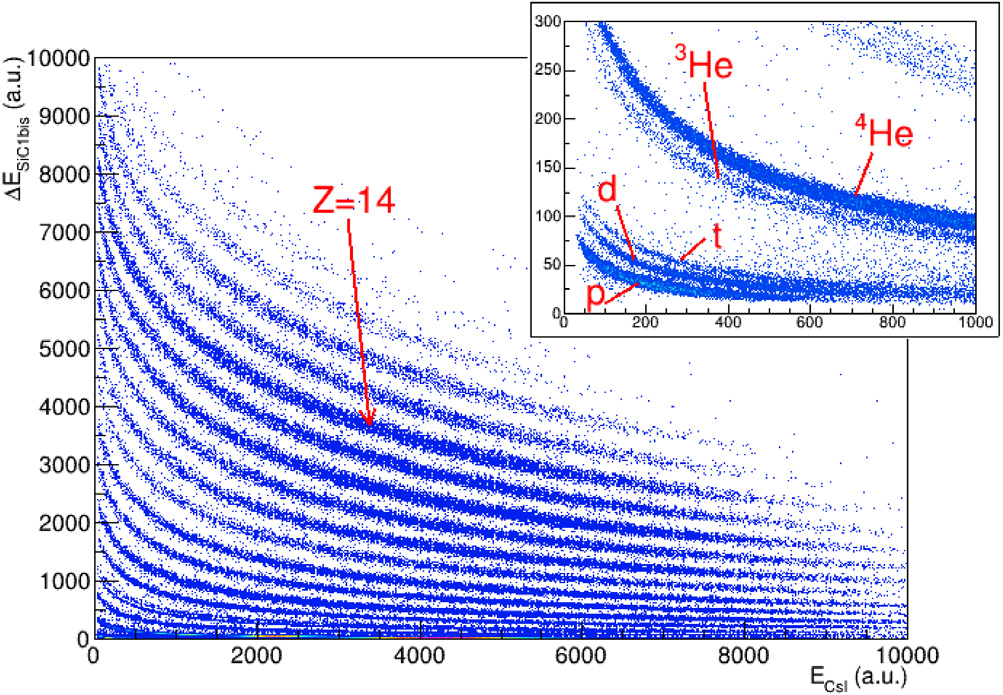
\includegraphics[width=\textwidth, keepaspectratio]{Grafici/ciampi-deltaE-E.png}
	\caption{Le correlazione $\Delta E - E_{resid}$ ottenute con il telescopio SiC-CsI in Figura~\ref{fig:ciampi_telescopio}. Il riquadro nell'angolo in alto a destra mostra uno zoom della regione con $Z \lesssim 2$. Figura tratta da~\cite{ciampi:nima19}.} \label{fig:ciampi_deltaE_E}
\end{figure}

%La resistenza alle radiazioni dei rivelatori al SiC è stata indagata sia attraverso simulazioni Monte Carlo sia per mezzo di test sperimentali. 
%Poiché la resistenza alle radiazioni è l'aspetto di maggiore importanza per la scelta dei dispositivi da utilizzare per NUMEN, alcune simulazioni Monte Carlo sono state implementate allo scopo di darne una stima nel caso dei rivelatori al SiC. 
%In Figura~\ref{fig:sic_simul_resist_radiaz} (a sinistra) sono riportati i risultati della produzione di vacanze generata da protoni e \ce{^{18}O} in un rivelatore da 100~$\mu$m.
%Come si può notare, i difetti causati dagli ioni di ossigeno sono due ordini di grandezza maggiori di quelli indotti dai protoni.
%Un andamento simile si osserva anche per la corrente inversa, mostrata in Figura~\ref{fig:sic_simul_resist_radiaz} (a destra). Sebbene questa aumenti di diversi ordini di grandezza dopo alte dosi di irradiazione, può essere ancora tollerabile, essendo cinque ordini di grandezza inferiore a quella del silicio.

%La resistenza alle radiazioni di rivelatori al SiC di piccole dimensioni ($2 \times 2$~mm\ap{2}, 30~$\mu$m di spessore) è stata analizzata in un test in cui i dispositivi erano irraggiati con ioni pesanti~\cite{raciti:npa10}. 
Dal momento che la resistenza alle radiazioni è un aspetto essenziale per la scelta dei dispositivi da utilizzare per NUMEN, è stata svolta un'attenta ricerca bibliografica per cercare dati sperimentali sul comportamento del SiC quando viene sottoposto ad elevate dosi di radiazioni.
%Da tale ricerca è emerso che su rivelatori di piccole dimensioni ($2 \times 2$~mm\ap{2}, 30~$\mu$m di spessore) è stato condotto un test in cui i dispositivi erano irraggiati con ioni pesanti~\cite{raciti:npa10}.
%Dalla ricerca è emerso che diversi studi sono stati condotti su tale argomento, i quali affermano concordemente che la robustezza del SiC è, a parità di condizioni, molto maggiore di quella del silicio~\cite{garcialopez:nimb16, nava:nima03}; in particolare, è stato realizzato un test su rivelatori di piccole dimensioni ($2 \times 2$~mm\ap{2}, 30~$\mu$m di spessore) in cui i dispositivi erano irraggiati con ioni pesanti~\cite{raciti:npa10}.
%I risultati hanno dimostrato che tali rivelatori sono in grado di sostenere fluenze dell'ordine di $10^{14}$  $\mbox{ioni}/\mbox{cm}^2$.
Dalla ricerca è emerso che diversi studi sono stati condotti su tale argomento, i quali affermano concordemente che la robustezza del SiC è, a parità di condizioni, molto maggiore di quella del silicio~\cite{garcialopez:nimb16, nava:nima03}; in particolare, in un test~\cite{raciti:npa10} si è riscontrato che giunzioni Shottky in SiC possono sostenere fluenze dell'ordine $10^{14}$  $\mbox{ioni}/\mbox{cm}^2$, soddisfacendo uno dei principali requisiti di NUMEN.
Tuttavia, dal momento che tali studi sono stati condotti adoperando dispositivi con caratteristiche differenti da quelle previste per NUMEN (che prevede l'uso di giunzioni p-n), una campagna di test specifici è stata condotta.
I primi risultati confermano che anche in questo caso vengono preservate le proprietà di resistenza alle radiazioni. 

%\begin{figure} [!t]
%	\centering
%	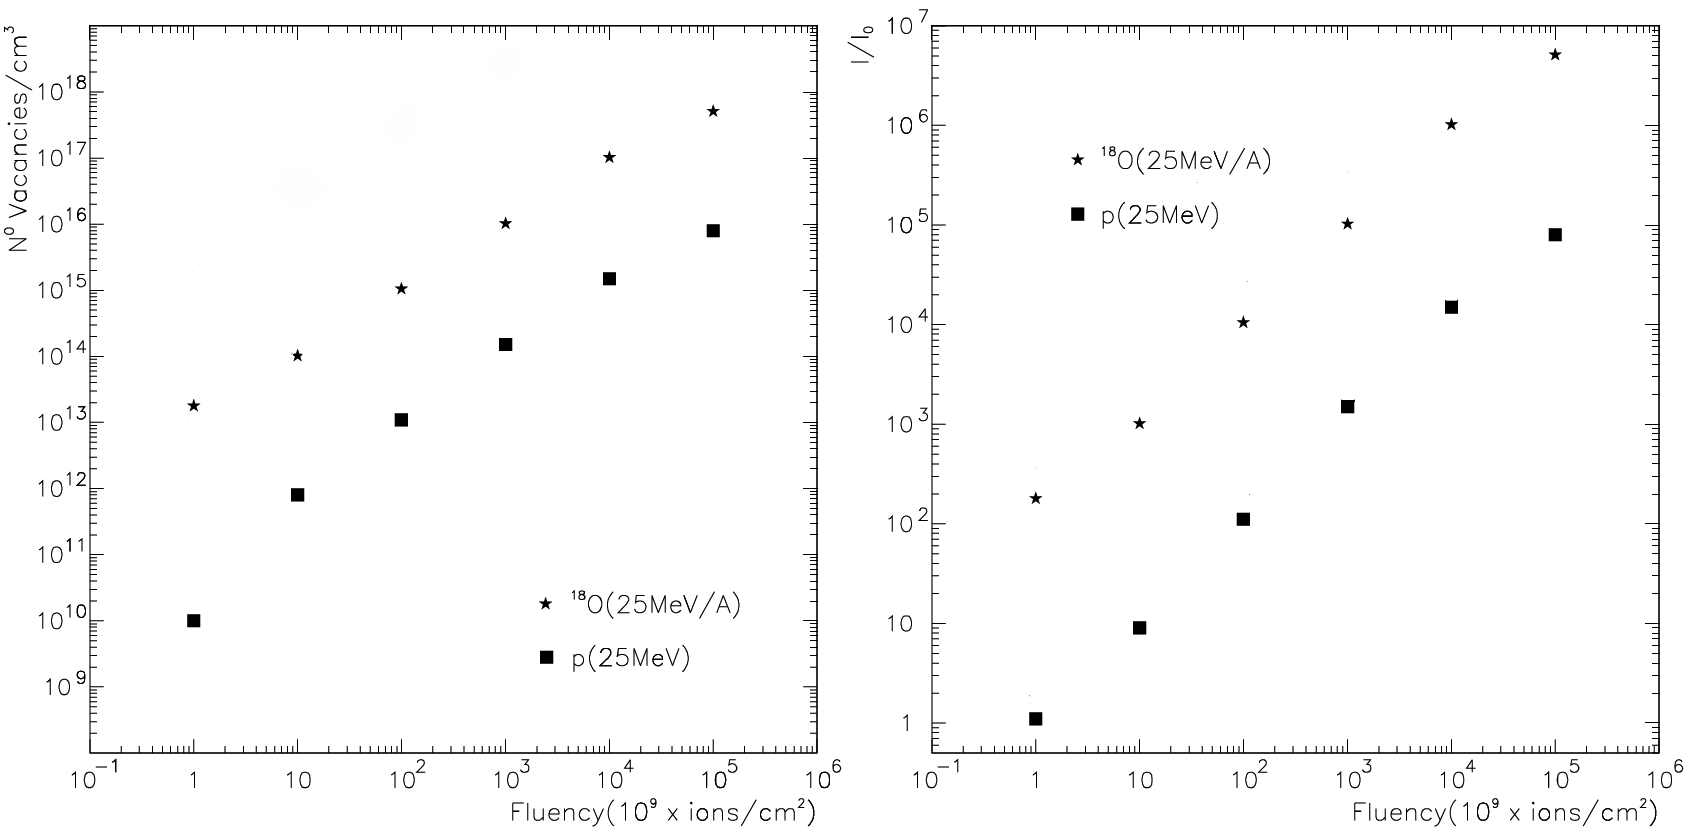
\includegraphics[width=\textwidth, keepaspectratio]{Grafici/sic_simul_resist_radiaz.png}
%	\caption{ Simulazioni Monte Carlo del numero di dislocamenti (a sinistra) e della corrente inversa (a destra) generati in un rivelatore al SiC da 100~$\mu$m in funzione della fluenza di protoni e \ce{^{18}O}. Figura tratta da~\cite{cappuzzello:epja18}.} \label{fig:sic_simul_resist_radiaz}
%\end{figure}



%Gli attuali limiti tecnologici alla produzione di rivelatori al SiC sono legati alla capacità di controllare le dimensioni dell'area attiva e lo spessore dei dispositivi, dal momento che essi vengono realizzati tramite crescita epitassiale su un substrato di SiC.
Gli attuali limiti tecnologici alla produzione di rivelatori al SiC sono legati alla capacità di fabbricare dispositivi con area attiva e spessori relativamente grandi, dal momento che essi vengono realizzati tramite crescita epitassiale su un substrato di SiC.
%Ciò comporta anche la presenza di una regione in cui la ... ZONA PARZIALMENTE VIVA .... NON SO BENE COME INTRODURLA 
Inoltre, la presenza di tale substrato potrebbe rappresentare un problema ai fini della rivelazione, in quanto costituisce uno strato morto in cui le particelle perdono energia senza che questa possa essere misurata o possono perfino fermarsi.
Grazie all'utilizzo di tecniche di ablazione LASER, il substrato potrebbe essere assottigliato fino a pochi~$\mu$m di spessore, ma tale operazione comporta un aumento dei costi, nonché una diminuzione dell'efficienza di produzione, in quanto alcuni dispositivi potrebbero venire danneggiati.
%Inoltre, poiché non è detto che la riduzione del substrato porti significativi benefici, 
Bisogna, dunque, ponderare l'effettiva utilità della riduzione del substrato.
%Tali problematiche sono state tenute in considerazione nella simulazione svolta per questo lavoro di tesi, la quale ne ha valutato l'impatto sulle performance del previsto sistema di rivelazione. 

La simulazione svolta per questo lavoro di tesi ha tenuto in considerazione tali limiti e problematiche, valutandone l'impatto sulle performance del sistema di rivelazione e suggerendo le specifiche tecniche ottimali ai fini del progetto. 






%I due prototipi di rivelatori al SiC utilizzati nel test sono mostrati in Figura~\ref{fig:sic}; essi avevano caratteristiche differenti: uno, chiamato \emph{SiC~A}, aveva un'area attiva non segmentata di $10 \times 10$~mm\ap{2}, con uno spessore di 10~$\mu$m ed uno strato morto di 100~$\mu$m; l'altro, indicato con \emph{SiC~B}, aveva un'area attiva segmentata in quattro pad, ciascuna di $5 \times 5$~mm\ap{2}, con uno spessore di 100~$\mu$m ed un strato morto di 350~$\mu$m.





%I due prototipi di rivelatori al SiC utilizzati nel test presentavano caratteristiche differenti: in primo luogo avevano spessore diversi, poiché uno era spesso 10~$\mu$m, mentre l'altro 100~$\mu$m.

%\vspace{0.5 cm}

\subsection{\iflanguage{italian}{Gli scintillatori allo ioduro di cesio}{Caesium iodide scintillation detector}}





%\subsection{\iflanguage{italian}{I telescopi SiC-CsI}{SiC-CsI telescope detectors}}
I rivelatori a scintillazione, detti anche \emph{scintillatori}, sono tra i più diffusi strumenti per la rivelazione delle particelle.
%Il loro principio di funzionamento è basato sul fatto che quando una particella carica attraversa uno scintillatore vengono emessi fotoni. 
%Il loro principio di funzionamento è basato sull'emissione di luce di scintillazione da parte di certi materiali quando attraversati da una particella carica
Il loro principio di funzionamento è il seguente: quando una particella carica attraversa uno scintillatore, eccita gli atomi o le molecole del materiale, i quali si diseccitano emettendo fotoni. 
La luce prodotta, proporzionale all'energia depositata nel mezzo, viene raccolta e trasformata in segnale elettrico da appositi sensori, come i fotomoltiplicatori o i fotodiodi.
Dal momento che l'energia media necessaria per la creazione di un fotone è circa trenta volte superiore a quella richiesta per la produzione di una coppia elettrone-lacuna in un semiconduttore, la risoluzione energetica tipica degli scintillatori è peggiore di quella dei rivelatori a semiconduttore.
%, con valori tipicamente compresi tra $1 \div 3 \%$.
%I due rivelatori al SiC sono stati assemblati insieme ai due scintillatori allo CsI mostrati in Figura~\ref{fig:csi}. 
%Fra le tipologie più diffuse di scintillatori, lo ioduro di cesio occupa uno dei posti più importanti.

Molti materiali possono produrre luce di scintillazione, differenziandosi per resa in luce, linearità e tempi di decadimento, laddove la resa in luce esprime il numero di fotoni prodotti per unità di energia depositata, la linearità descrive il rapporto di proporzionalità fra la resa in luce e l'energia depositata, il tempo di decadimento indica il tempo necessario per l'emissione di luce dopo il deposito di energia.
Uno dei materiali più diffusi per la realizzazione di rivelatori a scintillazione è lo CsI attivato al Tl, indicato solitamente come CsI(Tl). 
%Dal momento che possiede una fra le maggiori rese in luce e una notevole malleabilità, viene spesso impiegato nella rivelazione sia di particelle cariche sia di raggi gamma.
Dal momento che possiede una fra le maggiori rese in luce e una notevole malleabilità, negli ultimi cinquant'anni ha trovato un largo utilizzo negli esperimenti sia di fisica nucleare sia di fisica particellare, venendo impiegato nella rivelazione di particelle cariche o di raggi gamma.


%La resistenza alle radiazioni dei cristalli di CsI è stata largamente studiata
%Innumerevoli test sono stati condotti per valutare la resistenza alle radiazioni dei cristalli di CsI(Tl), 
%Uno degli aspetti che hanno contribuito alla diffusione dello CsI(Tl) (nel seguito indicato come CsI) è la sua resistenza alle radiazioni, che è stata oggetto di innumerevoli test~\cite{beylin:nima04}. I risultati sono concordi nell'affermare che, sebbene ci siano fluttuazioni legate alla purezza e alle dimensioni dei cristalli, la resa in luce non dovrebbe subire variazioni significative alle intensità di fascio che verranno utilizzate per NUMEN.
%
%Innumerevoli studi sono stati condotti per valutare la resistenza alle radiazioni dello CsI(Tl) (nel seguito indicato come CsI) utilizzando  
%La resistenza alle radiazioni dello CsI(Tl) (nel seguito indicato come CsI) è stata oggetto di innumerevoli test in cui i cristalli venivano irraggiati con raggi gamma o con elettroni.
Uno degli aspetti che ha contribuito alla diffusione dello CsI(Tl) (nel seguito indicato come CsI) è la sua resistenza alle radiazioni, che è stata oggetto di innumerevoli studi in cui i cristalli venivano irraggiati con raggi gamma o con elettroni~\cite{beylin:nima04, zhu:nima98}.
%I risultati sperimentali danno incoraggianti prospettive di sopravvivenza per i cristalli alle intensità di fascio che verranno utilizzate per NUMEN.
%I risultati sono concordi nell'affermare che, sebbene ci siano fluttuazioni legate alla purezza e alle dimensioni dei cristalli, la resa in luce non dovrebbe subire variazioni significative alle intensità di fascio che verranno utilizzate per NUMEN.
Tuttavia, dal momento che in letteratura non sono stati trovati dati sperimentali riguardo la sua resistenza agli ioni pesanti, la collaborazione NUMEN ha svolto specifici test sottoponendo un cristallo di CsI di $ 1 \times 1$~cm\ap{2} ad un fascio di \ce{^{14}N} a 65~AMeV, per una fluenza totale di circa $10^{12}$~particelle/cm\ap{2}, equivalente a circa due anni di esperimento.
Alla fine dell'irraggiamento, il cristallo non presentava danni visibili e la sua resa in luce non mostrava significative variazioni, come si può evincere dalla Figura~\ref{fig:spettro_csi}.
Supportati da questi incoraggianti risultati, la scelta di utilizzare lo CsI sembra promettere le capacità di resistenza alle radiazioni necessarie per NUMEN.

\begin{figure} [!p]
	\centering
	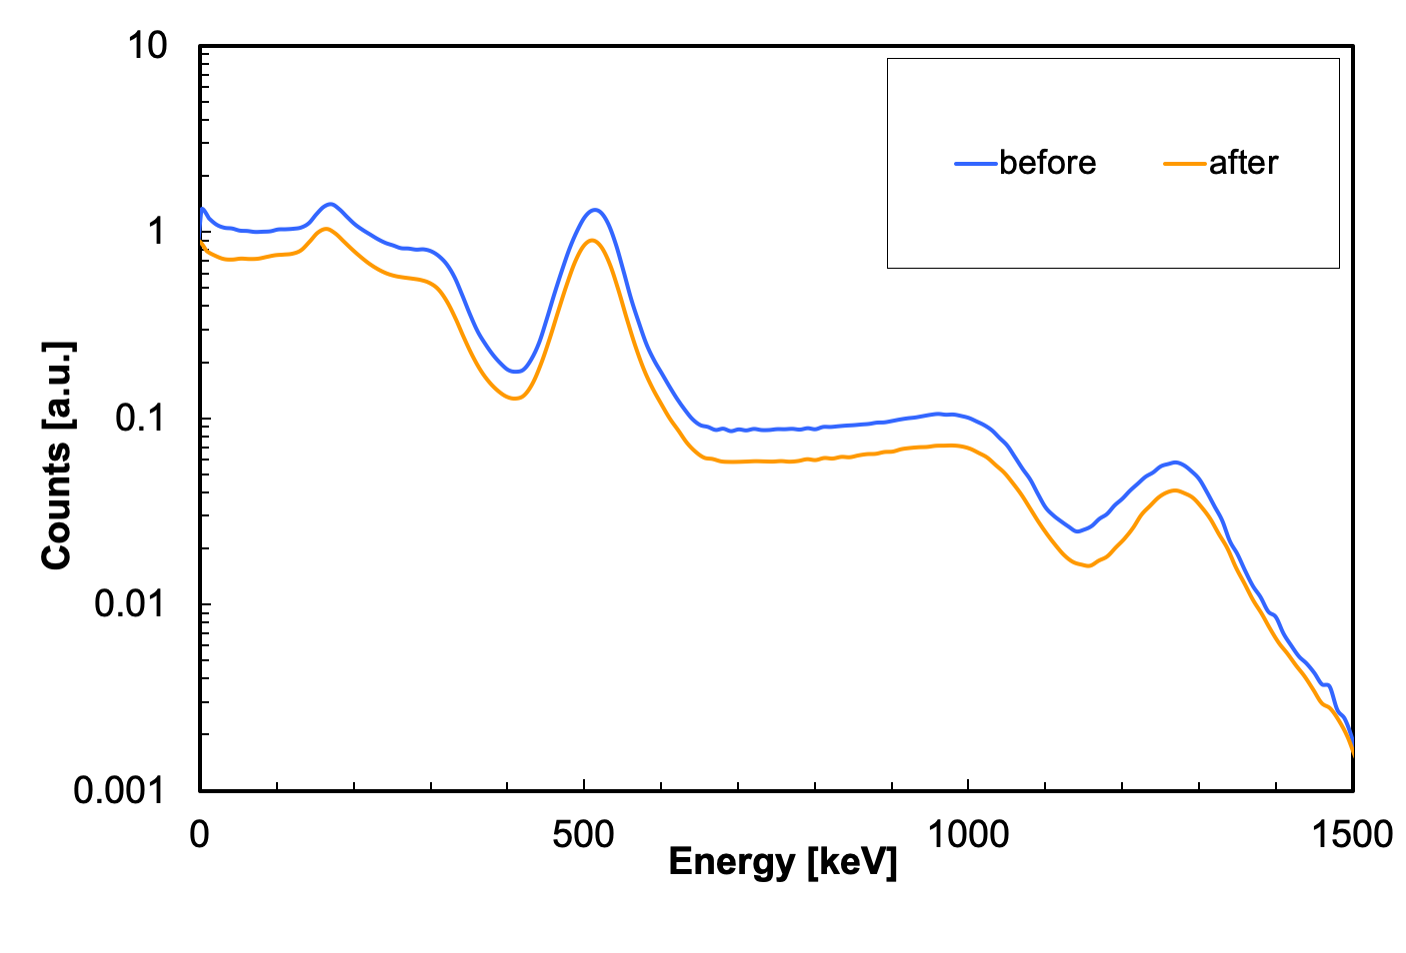
\includegraphics[width=\textwidth, keepaspectratio]{Grafici/spettro_csi.png}
	\caption{Spettro energetico misurato con uno scintillatore allo CsI, prima (blu) e dopo (arancione) un irraggiamento equivalente a circa due anni di esperimento NUMEN.} \label{fig:spettro_csi}
\end{figure}




%\clearpage

%\vspace{0.5 cm}

%\section{\iflanguage{italian}{La configurazione dell'apparato sperimentale nel test}{Experimetal apparatus setting}}
\section{\iflanguage{italian}{Il test beam sui telescopi}{Telescope detectors experimental test}} \label{sez:test}

% ******** QUESTA ERA LA PARTE CHE SECONDO ME VA BENE PER INTRODURRE IL TEST
Ad Aprile 2019 i primi due prototipi di rivelatori al SiC per il progetto NUMEN sono stati completati e resi disponibili dalla ST-Microelectronics. Dal momento che tali dispositivi non sono ancora uno standard nel mondo della fisica ma rappresentano una tecnologia di frontiera, è stato condotto un test per analizzarne la risposta nelle condizioni sperimentali tipiche della Fase~2.
%; una buona risoluzione energetica dello stadio $\Delta E$ di un telescopio è, infatti, essenziale per avere delle buone capacità di PID.

Lo scopo principale del test era valutare la capacità di PID dei telescopi SiC-CsI per gli ioni di interesse, confrontandola con quella dell'attuale sistema basato, sulla combinazione di fili proporzionali e rivelatori al silicio.
%valutandone la capacità di PID nella regione di interesse per NUMEN e confrontandola con quella accessibile con l'attuale apparato. 
%Come illustrato nel Paragrafo~\ref{sez:sistema_identif_part}, i rivelatori al SiC sono stati scelti nell'ambito del progetto come stadio~$\Delta E$ di un telescopio SiC-CsI per l'identificazione in numero atomico dei prodotti di reazione. Lo scopo principale del test era, dunque, valutare la capacità di PID di questo sistema nella regione di interesse per NUMEN, confrontandola con quella accessibile con l'attuale apparato.
In aggiunta, poiché l'upgrade del FPD prevede anche la sostituzione dell'elettronica attualmente utilizzata con una basata su chip VMM3a~\cite{degeronimo:ieee13}, il test aveva anche l'obiettivo di valutare le prestazioni del primo prototipo di elettronica di front-end prevista per NUMEN.
Ciò ha, inoltre, permesso di effettuare un confronto delle performance dei telescopi in funzione dell'elettronica adoperata.

Il test è stato svolto ai LNS utilizzando un fascio di~\ce{^{20}Ne} a 20~AMeV, incidente su \ce{^{197}Au} o \ce{^{12}C}, laddove i due bersagli avevano funzioni differenti: il primo serviva per massimizzare eventi di scattering elastico, il secondo per favorire la formazione dei prodotti di reazione di interesse.
%, ovvero quella dell'O, del F e del Ne.




%\vspace{0.5 cm}


\subsection{\iflanguage{italian}{I telescopi utilizzati nel test}{Telescope detectors used in the test}}

\begin{figure} [!p]
	\centering
	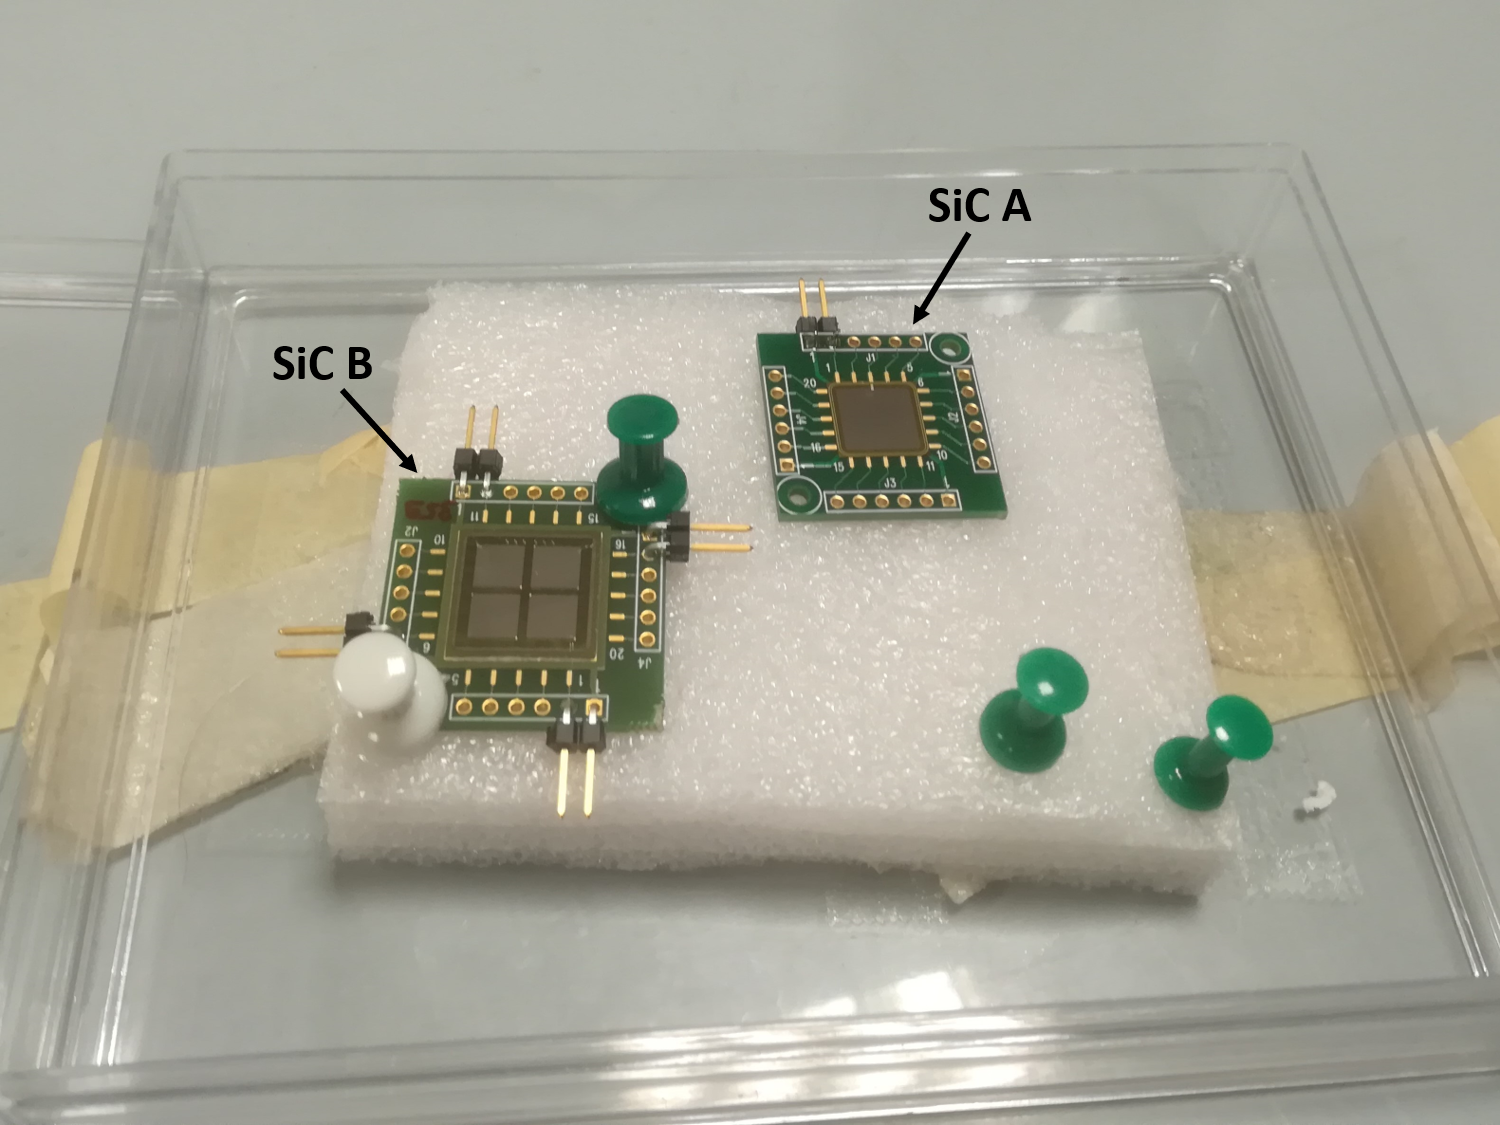
\includegraphics[width=\textwidth, keepaspectratio]{Grafici/sic_etichette.png}
	\caption{I rivelatori al carburo di silicio (SiC) utilizzati nel test: a sinistra il \emph{SiC~B}, a destra il \emph{SiC~A}.} \label{fig:sic}
\end{figure}

I due prototipi di rivelatori al SiC utilizzati nel test sono mostrati in Figura~\ref{fig:sic}: come è possibile notare, essi differiscono innanzitutto per la segmentazione dell'area attiva, in quanto uno (\emph{SiC~A}) è costituito da un'unica pad, mentre l'altro (\emph{SiC~B}) è suddiviso in quattro regioni. 
%Inoltre, mentre il SiC~A aveva un'area attiva di $10 \times 10$~mm\ap{2}, il SiC~B presentava 
%I due telescopi SiC-CsI utilizzati nel test
Entrambi i rivelatori hanno un'area attiva complessiva di $10 \times 10$~mm\ap{2}, laddove ogni pad del SiC~B ha un'estensione di $5 \times 5$~mm\ap{2}.
%Un'ulteriore differenza riguardava gli spessori dei due rivelatori: mentre il SiC~A era spesso 10~$\mu$m con 100~$\mu$m di strato morto, il SiC~B aveva uno spessore di 100~$\mu$m con 350~$\mu$m di .
Un'ulteriore differenza riguarda lo spessore della regione attiva dei due rivelatori: per il SiC~A è di 10~$\mu$m, mentre per il SiC~B misura 100~$\mu$m.
Infine, entrambi i rivelatori hanno un substrato morto, che per il SiC~A è spesso 100~$\mu$m, invece per il SiC~B ha uno spessore di~350~$\mu$m.
In occasione del test si è scelto di utilizzare soltanto due delle quattro pad del SiC~B, le quali sono state cortocircuitate tra loro in modo che questo rivelatore avesse una superficie sensibile di $10 \times 5$~mm\ap{2}.





%\vspace{3 cm}


\begin{figure} [!t]
	\centering
	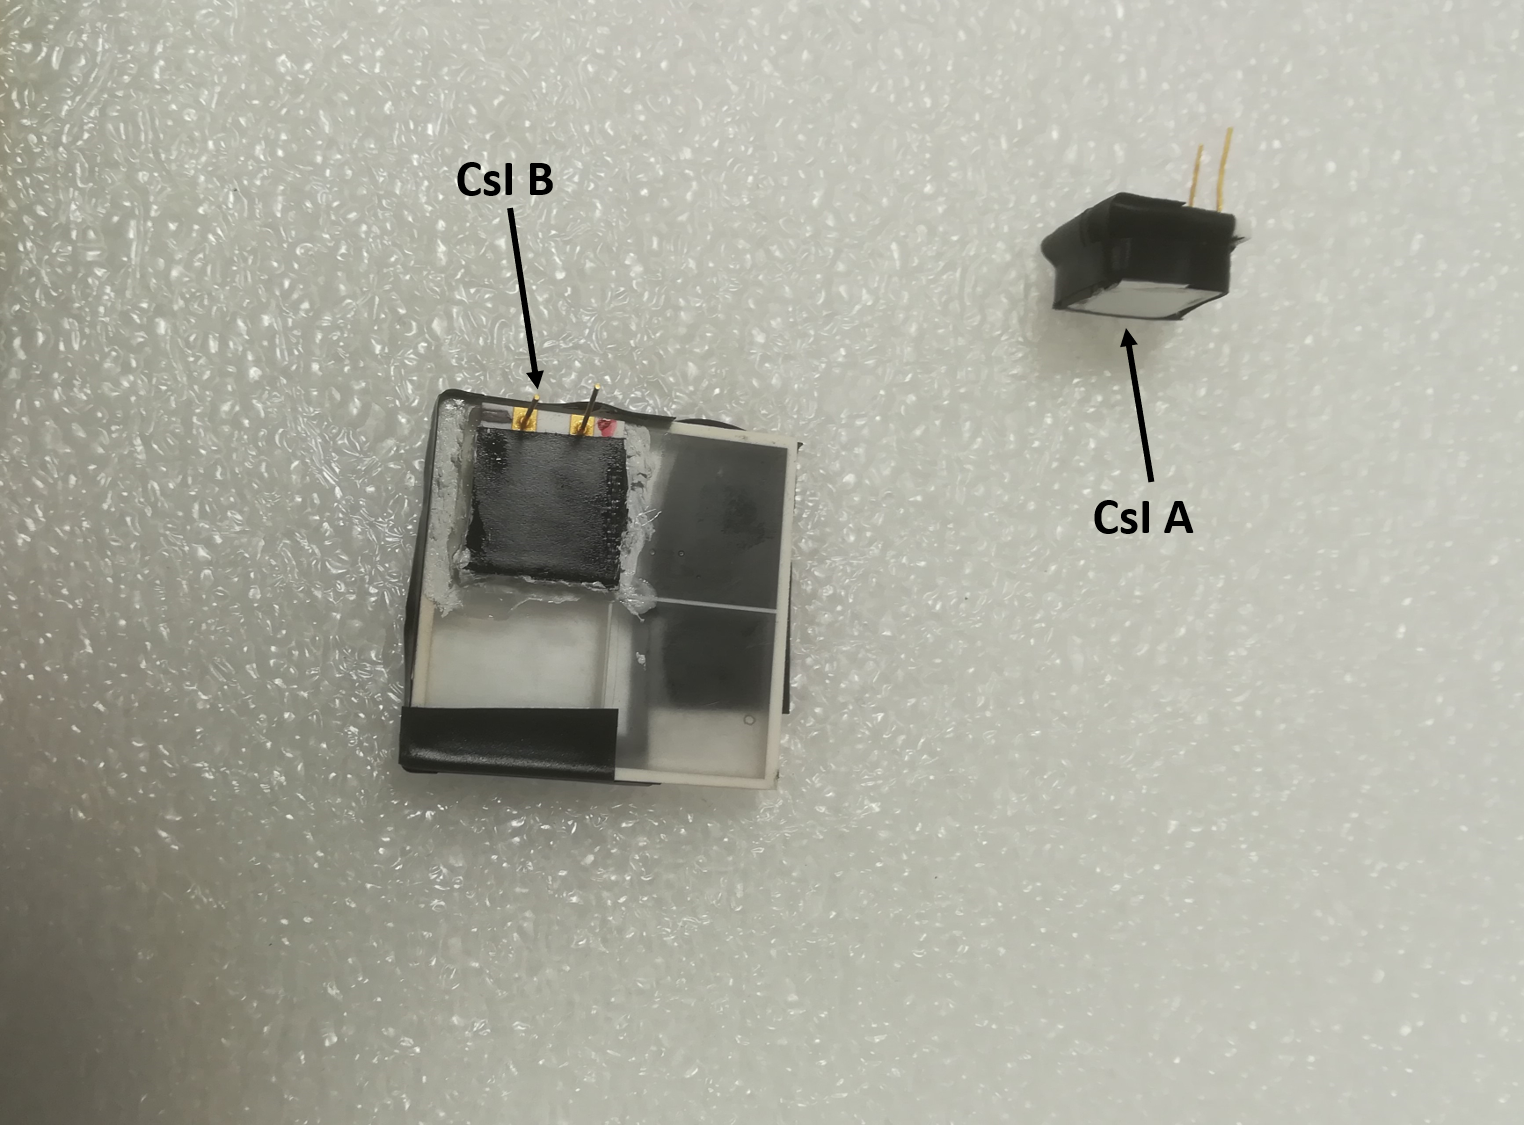
\includegraphics[scale=0.5]{Grafici/csi_etichette.png}
	\caption{I rivelatori a scintillazione utilizzati nel test: a sinistra il \emph{CsI~B}, a destra il \emph{CsI~A}. Guardando, ad esempio, il CsI~B, si possono notare lo scintillatore (CsI), che appare come un materiale trasparente, e il fotodiodo, che si trova coperto dal nastro isolante nero per migliorare la schermatura. Inoltre, è possibile vedere anche il Mylar bianco con cui sono stati rivestiti i cristalli.} \label{fig:csi}
\end{figure}



%In occasione del test sono stati utilizzati due scintillatori allo CsI, i quali sono mostrati in Figura~\ref{fig:csi}.
Gli scintillatori allo CsI utilizzati nel test sono mostrati in Figura~\ref{fig:csi}.
Essi hanno dimensioni differenti: uno (\emph{CsI~A}) è da $1 \times 1$~cm\ap{2}, l'altro (\emph{CsI~B}) è suddiviso in quattro regioni da $1.5 \times 1.5$~cm\ap{2}. 
%La luce di scintillazione veniva letta in entrambi i casi con un fotodiodo da $1 \times 1$~cm\ap{2}, che 
%Ognuno dei due scintillatori era accoppiato ad un fotodiodo $1 \times 1$~cm\ap{2}
A causa delle dimensioni dei rivelatori al SiC, soltanto una delle quattro aree sensibili del CsI~B è stata utilizzata. Per migliorare la raccolta della luce, i cristalli sono stati avvolti con del Mylar bianco, il quale è stato fissato con del nastro isolante nero.
%
%I cristalli sono stati avvolti con del mylar e del nastro isolante nero per migliorare la raccolta della luce.
%
Ciascuno scintillatore era accoppiato tramite grasso ottico ad un fotodiodo di area $1 \times 1$~cm\ap{2} per la lettura della luce di scintillazione. 



\begin{figure} [!t]
	\centering
	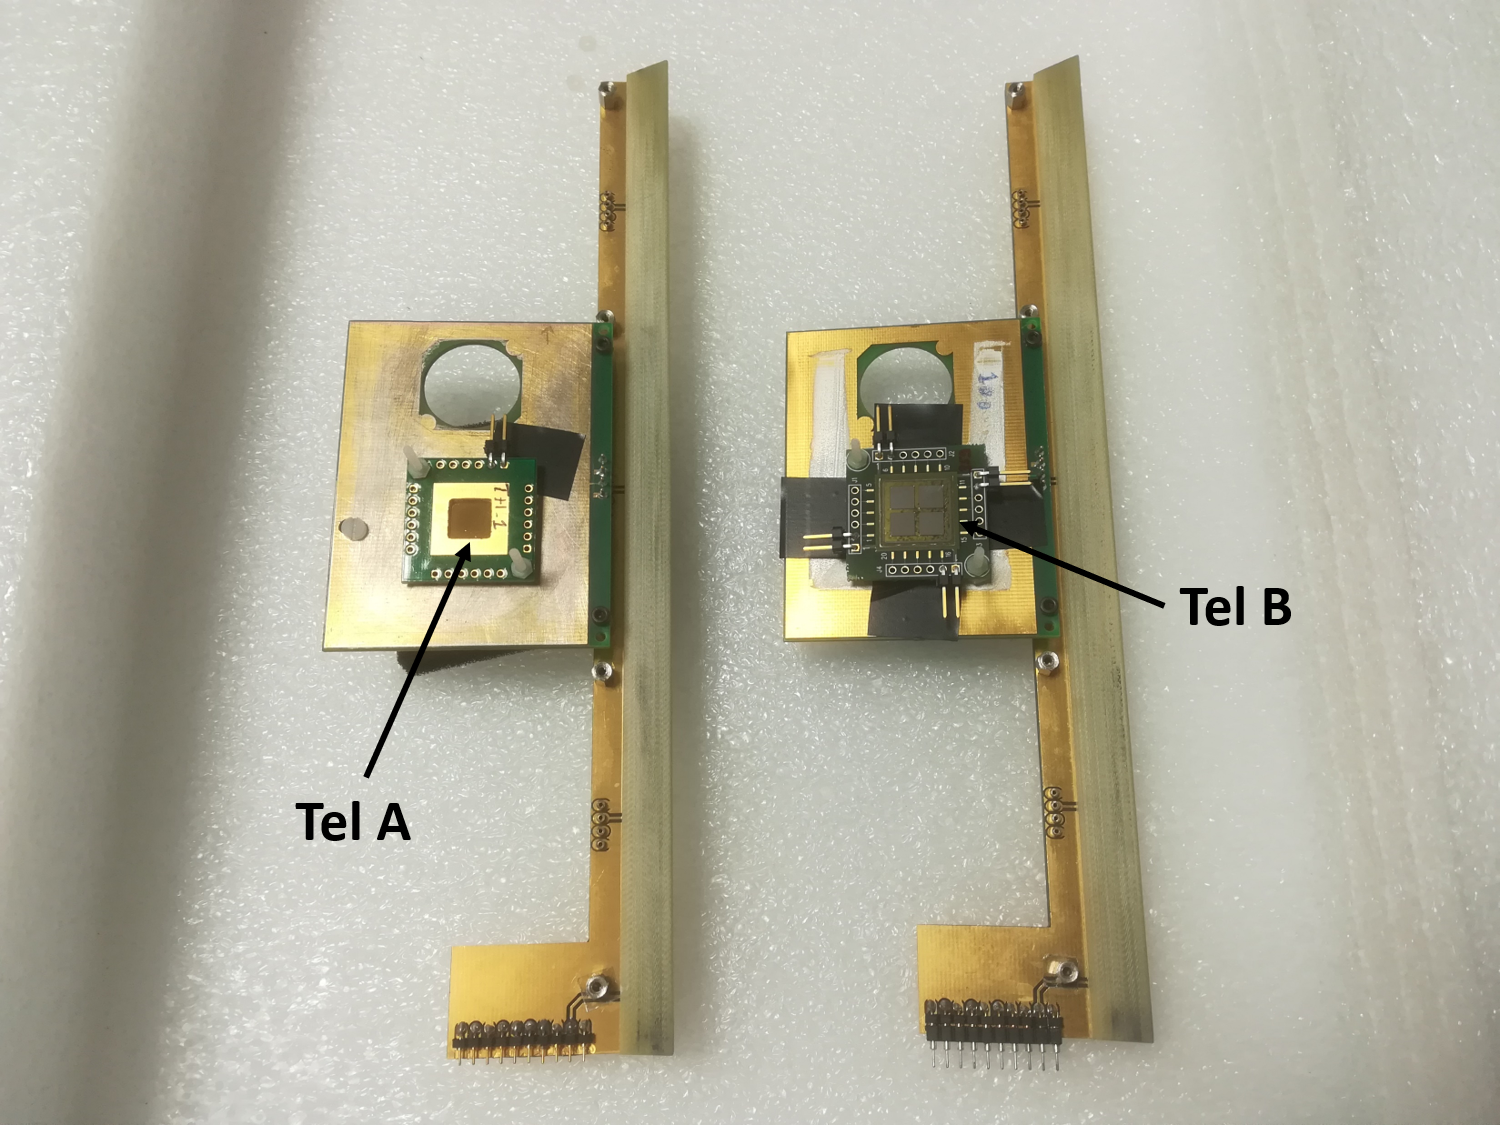
\includegraphics[scale=0.5]{Grafici/telescopi_etichette.png}
	\caption{I due telescopi SiC-CsI utilizzati nel test: a sinistra il \emph{Tel~A}, a destra il \emph{Tel~B}.} \label{fig:telescopi}
\end{figure}






Il SiC~A e il SiC~B sono stati assemblati, rispettivamente, con il CsI~A e il CsI~B, così da formare i due telescopi (\emph{Tel~A} e \emph{Tel~B}) mostrati in Figura~\ref{fig:telescopi}.
%; in particolare, mentre nel Tel~A il SiC~A era \emph{reverse mounted}, nel Tel~B il SiC~B era \emph{direct mounted} (\textcolor{red}{va bene detto così?}).
Al fine di ottenere una migliore correlazione $\Delta E - E_{resid}$, il SiC~A è stato montato in configurazione \emph{reverse}, ovvero rivolgendo alle particelle incidenti prima il substrato morto e poi la regione sensibile.
Ciò non è stato possibile per il SiC~B a causa del maggiore substrato morto che avrebbe fermato gli ioni.
%I due telescopi, fissati su due delle strutture che solitamente ospitano i rivelatori al silicio, sono stati posti nel FPD secondo lo schema riportato in Figura.
%Come si può notare, quattro rivelatori al silicio sono stati montati in modo simmetrico rispetto al SiC~A, in modo da avere un utile riferimento sia per la fase di acquisizione sia per l'analisi offline.
%Come si può notare, a sinistra e a destra del Tel~A sono stati montati due rivelatori al silicio, in modo da avere un utile riferimento sia per la fase di acquisizione sia per l'analisi offline.
Dunque, all'energia utilizzata nel test, gli ioni incidenti sul Tel~B venivano arrestati nel substrato del SiC~B, per cui da questo telescopio era possibile estrarre soltanto l'informazione sul $\Delta E$.

I due telescopi, fissati su schede in PCB, sono stati posti nel FPD di MAGNEX in due delle colonne che solitamente ospitano i rivelatori al silicio.
%A sinistra e a destra del Tel~A sono stati montati due rivelatori al silicio, in modo da avere un utile riferimento sia per la fase di acquisizione sia per l'analisi offline.
Insieme ai due telescopi sono stati montati quattro rivelatori al silicio: due erano posizionati fra il Tel~A e il Tel~B, e due a sinistra del Tel~A.
Questi avevano lo scopo di fornire un riferimento durante l'acquisizione dei dati sperimentali ed essere un metro di paragone per le capacità di PID in fase di analisi.









%\subsection{\iflanguage{italian}{Configurazione dell'apparato sperimentale}{Setting of the experimental apparatus}}
\subsection{\iflanguage{italian}{Le catene elettroniche del test}{The electronic chains used in the test}}


%La catena elettronica 
%Dal momento che il test aveva anche lo scopo di valutare le differenze di risposta dei telescopi SiC-CsI a seconda dell'elettronica utilizzata, sono state montate due diverse catene elettroniche:
Dal momento che il test aveva anche lo scopo di valutare le differenze di risposta dei telescopi SiC-CsI a seconda dell'elettronica utilizzata, il Tel~A è stato equipaggiato con due diverse catene elettroniche:
la prima (\emph{standard}) rispecchia quella attualmente adoperata per i rivelatori al silicio, la seconda (\emph{VMM3a}) era incentrata sul prototipo di chip VMM3a.
%, a cui ci si riferisce come \emph{elettronica~Boiano} nel caso dell'elettronica attualmente adoperata e come \emph{elettronica~VMM3} nel caso di quella prevista per NUMEN.
%La catena elettronica del sistema fili+silici non è discussa nel presente lavoro di tesi
%Dunque, nel presente lavoro di tesi viene
I fili proporzionali e i rivelatori al silicio utilizzati nel test hanno, invece, montato l'elettronica tradizionale, la quale, essendo stata ampiamente discussa in numerose pubblicazioni, non verrà illustrata nel presente lavoro di tesi.
%Poiché l'elettronica standard di MAGNEX è stata ampiamente discussa in numerose pubblicazioni, nel presente lavoro di tesi vengono illustrate soltanto le catene elettroniche relative al Tel~A.
%Il tracciatore a gas e i rivelatori al silicio utilizzati nel test hanno montato la catena elettronica standard, di cui nel presente lavoro di tesi 
Dunque, nel seguito verranno descritte soltanto le due catene elettroniche relative al Tel~A.
%In entrambe le configurazioni, il trigger per l'acquisizione del segnale del telescopio era fornito dal CsI~A, il quale era inviato 

%È bene precisare che, mentre per i rivelatori al silicio sono stati usati PA da 5~mV/MeV, per il rivelatore al SiC e per lo scintillatore allo CsI sono stati utilizzati PA da 45~mV/MeV. 


%Nella catena elettronica standard, di cui in Figura si riporta uno schema, il segnale proveniente dal rivelatore era inviato ad un preamplificatore (PA) di carica~\cite{boiano:ieee08}.
%Sia per il rivelatore al SiC sia per lo scintillatore allo CsI sono stati utilizzati PA con sensibilità di 45~mV/MeV.
%Nella catena elettronica standard, di cui in Figura si riporta uno schema, i segnali provenienti dai due stadi del telescopio erano rispettivamente inviati a due preamplificatori (PA) di carica~\cite{boiano:ieee08} con sensibilità di 45~mV/MeV.

\paragraph{Elettronica standard} 
Nella catena elettronica standard, di cui in Figura~\ref{fig:elettronica_standard} si riporta uno schema, il segnale proveniente dal SiC~A era inviato ad un preamplificatore (PA) di carica~\cite{boiano:ieee08} con sensibilità di 45~mV/MeV.
Questo, oltre a raccogliere ed integrare il segnale, era utilizzato anche per fornire la tensione di alimentazione al rivelatore, pari a $-50$~V, generata da un alimentatore esterno.
%L'output del PA era collegata ad un amplificatore MEGAMP.
%L'uscita del MEGAMP era inviata all'ADC per l'acquisizione.
%L'output del PA era collegato ad un amplificatore MEGAMP a 16 canali, che, oltre ad amplificare il segnale, ne modificava la forma in modo da renderlo gaussiano.
%L'output del PA era collegato ad un amplificatore formatore MEGAMP a 16 canali, il quale possedeva due tipologie di uscite: una restituiva un segnale analogico,  impiegato per la misura dell'energia, l'altra produceva un segnale logico da discriminatore a frazione costante (Constant Fraction Discriminator, CFD), solitamente utilizzato per misure di tempo o per la creazione del gate.
L'output del PA era collegato ad un amplificatore formatore MEGAMP a 16 canali, il quale in un unico modulo riunisce amplificatore e discriminatore a frazione costante (Constant Fraction Discriminator, CFD); esso, infatti, possiede per ogni ingresso due tipologie di uscita: una restituisce un segnale analogico, tipicamente impiegato per la misura dell'energia, l'altra produce un segnale logico, solitamente utilizzato per misure di tempo o per la creazione del gate.
%
%
%Mentre la prima è tipicamente impiegata per la spettroscopia, 
%L'uscita del PA era, infine, inviata all'ADC per l'acquisizione dell'informazione sulla perdita di energia~$\Delta E$.
%Dal MEGAMP veniva, in questo caso, prelevato soltanto il segnale analogico, il quale, formato con uno shaping time di 500~ns.
In questo ramo della catena, dal MEGAMP veniva prelevato soltanto il segnale analogico, per il quale si era scelto uno shaping time di 500~ns.
Tale segnale era, infine, inviato all'ADC di picco per l'acquisizione dell'informazione sulla perdita di energia~$\Delta E$.
%
%Il segnale prodotto dal fotodiodo era collegato ad un PA analogo a quello utilizzato per il rivelatore al SiC.
%Dal momento che il segnale dello scintillatore era utilizzato per dare il trigger,

Per quanto riguarda il CsI~A, il segnale di output del fotodiodo era raccolto da un PA analogo a quello utilizzato per il SiC~A.
La tensione di alimentazione del fotodiodo, pari a $-70$~V, era fornita, anche in questo caso, tramite il PA e generata da un alimentatore esterno.
L'uscita del PA era inviata al MEGAMP, da cui venivano estratti due segnali: quello analogico era inviato direttamente all'ADC di picco per l'acquisizione dell'energia residua $E_{resid}$, quello del CFD veniva sdoppiata in due copie, di cui una era utilizzata per dare il gate all'acquisizione dei segnali del telescopio, mentre l'altra era inviata al modulo OR che produce il Master Trigger per l'acquisizione. 
A tale modulo erano collegati anche i segnali logici provenienti dalle catene elettroniche dei quattro rivelatori al silicio, in modo da consentire un'acquisizione parallela dei segnali standard di MAGNEX e di quelli del telescopio.

%utilizzato per dare il trigger all'acquisizione dei segnali del telescopio.

\begin{figure} [!p]
	\centering
	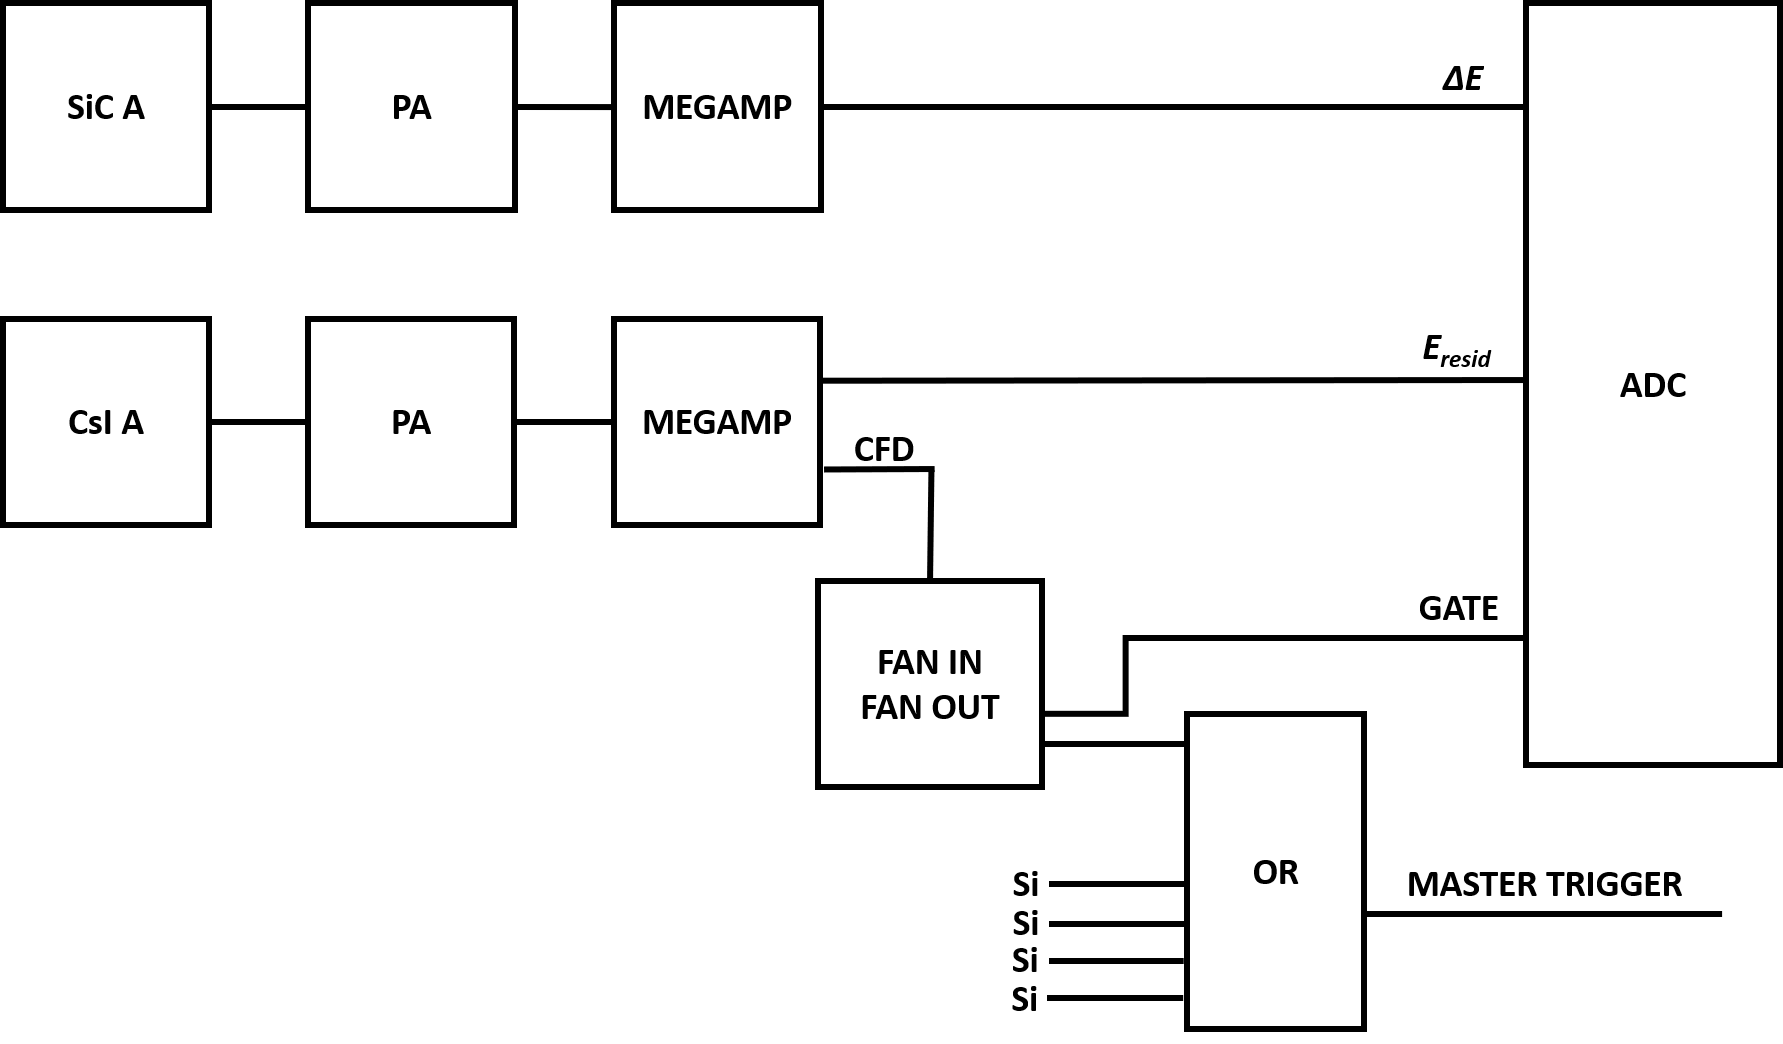
\includegraphics[width=\textwidth, keepaspectratio]{Grafici/elettronica_standard.png}
	\caption{L'elettronica \emph{standard} associata al Tel~A.} \label{fig:elettronica_standard}
\end{figure}

%\clearpage


\paragraph{Elettronica VMM3a} 
%Nella catena elettronica VMM3, il cui schema è illustrato in Figura~\ref{fig:elettronica_vmm}, il segnale del SiC~A era inviato direttamente al chip VMM3, il quale racchiudeva in sé un PA da $3 \div 6$~mV/fC e un amplificatore formatore con shaping time da 200~ns.
%
Nella catena elettronica VMM3a, il cui schema è illustrato in Figura~\ref{fig:elettronica_vmm}, il segnale del SiC~A era inviato direttamente al chip VMM3a, che, sviluppato in origine per l'esperimento ATLAS, è stato adattato per gli scopi di NUMEN.
Possedendo un'architettura a 64~canali, esso consente una più semplice gestione di apparati con un grande numero di canali.
%
%
%Tale chip possiede 64 canali e, per ogni canale, è capace di fornire informazioni sull'ampiezza del picco e sul timing del segnale. 
%La sensibilità del PA poteva essere selezionata nel range $3 \div 6$~mV/fC. 
%Tale chip possedeva un'architettura a 64~canali, consentendo, dunque, una più semplice gestione di apparati con un grande numero di canali.
Dal momento che il futuro muro per la PID prevede l'utilizzo di 1230 telescopi, la scelta di un'elettronica di front-end con questo tipo di caratteristiche è essenziale in termini di facilità di controllo dei dispositivi, di economia degli spazi e di più semplice dissipazione del calore.
%Per ogni canale, il chip poteva restituire l'informazione sul canale di provenienza, sull'ampiezza del picco e sul timing del segnale.
Per ogni canale il chip racchiude in sè un PA da $3 \div 6$~mV/fC e un amplificatore formatore con shaping time da $25 \div 200$~ns.
La scheda è, inoltre, dotata di un'uscita monitor, attraverso la quale è possibile osservare il segnale analogico formato dal circuito amplificatore.

Il VMM3a era collegato alla scheda di read-out System On Module (SOM) della National Instruments~\cite{national_instruments}.
%, che univa un efficace Field Programmable Gate Array (FPGA) ad un potente processore.
%Il compito principale della SOM era la lettura veloce dei segnali provenienti dal VMM3
Nella prospettiva della Fase~4, la SOM deve assicurare la lettura veloce dei segnali provenienti dal VMM3a e il trasferimento rapido dei dati al sistema di acquisizione tramite una connessione Gb~Ethernet.
Tali obiettivi saranno possibili grazie alla struttura della SOM, che unisce un efficace Field Programmable Gate Array (FPGA) ad un potente processore.
In Figura~\ref{fig:vmm+som} è riportata una foto del chip VMM3a e della scheda SOM utilizzati nel test.

Dal momento che all'oscilloscopio si era notato che il segnale di output della SOM era in anticipo rispetto al gate (dato dal CsI~A), il primo era inviato ad una linea di ritardo passiva da 140~ns. Infine, il segnale giungeva all'ADC per l'acquisizione.

%Il segnale di output della SOM, opportunamente ritardato di 140~ns, era inviato all'ADC, dove veniva acquisito.

Per quanto concerne il CsI~A, il segnale del fotodiodo era inviato al VMM3a, da cui, in questo caso, venivano estratti due segnali: uno, analogico, era dato in input alla SOM, l'altro, logico, veniva utilizzato per la formazione del gate. 
Poiché l'ADC utilizzata richiedeva in ingresso un gate negativo mentre il segnale logico prodotto dalla SOM era positivo, quest'ultimo era prima inviato ad un modulo Fan~in/Fan~out, da cui si prelevava l'uscita invertente (INV).
Dal momento che l'inversione del segnale richiedeva del tempo di elaborazione, il segnale analogico risultava in anticipo rispetto al gate. Anche in questo caso è stato, dunque, necessario ritardare opportunamente il segnale di output della SOM prima di inviarlo all'ADC.
Un'altra copia del segnale del CFD era inviata al modulo OR utilizzato per la generazione del Master Trigger, nel quale, come nella configurazione precedentemente discussa, giungevano anche i segnali logici delle catene dei rivelatori al silicio.
Pertanto, anche in questo set-up venivano registrati i segnali standard di MAGNEX.

\begin{figure} [!p]
	\centering
	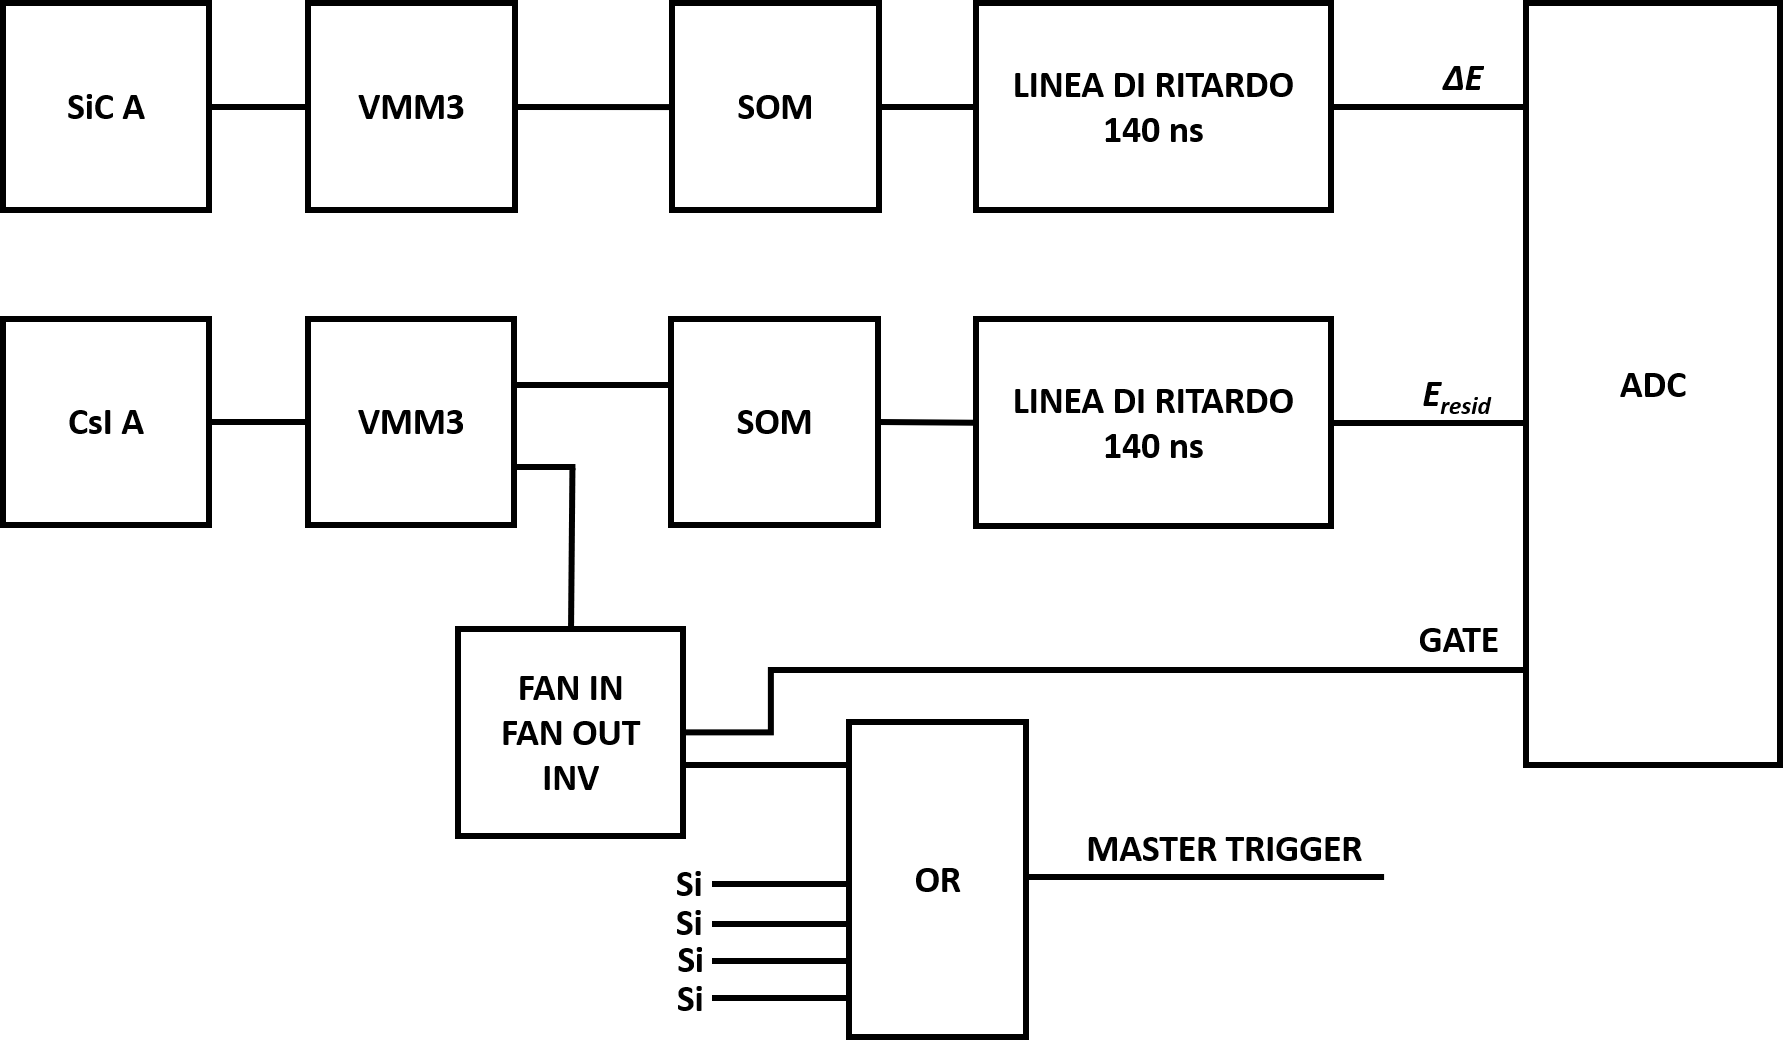
\includegraphics[width=\textwidth, keepaspectratio]{Grafici/elettronica_vmm.png}
	\caption{L'elettronica \emph{VMM3a} associata al Tel~A.} \label{fig:elettronica_vmm}
\end{figure}

\begin{figure} [!p]
	\centering
	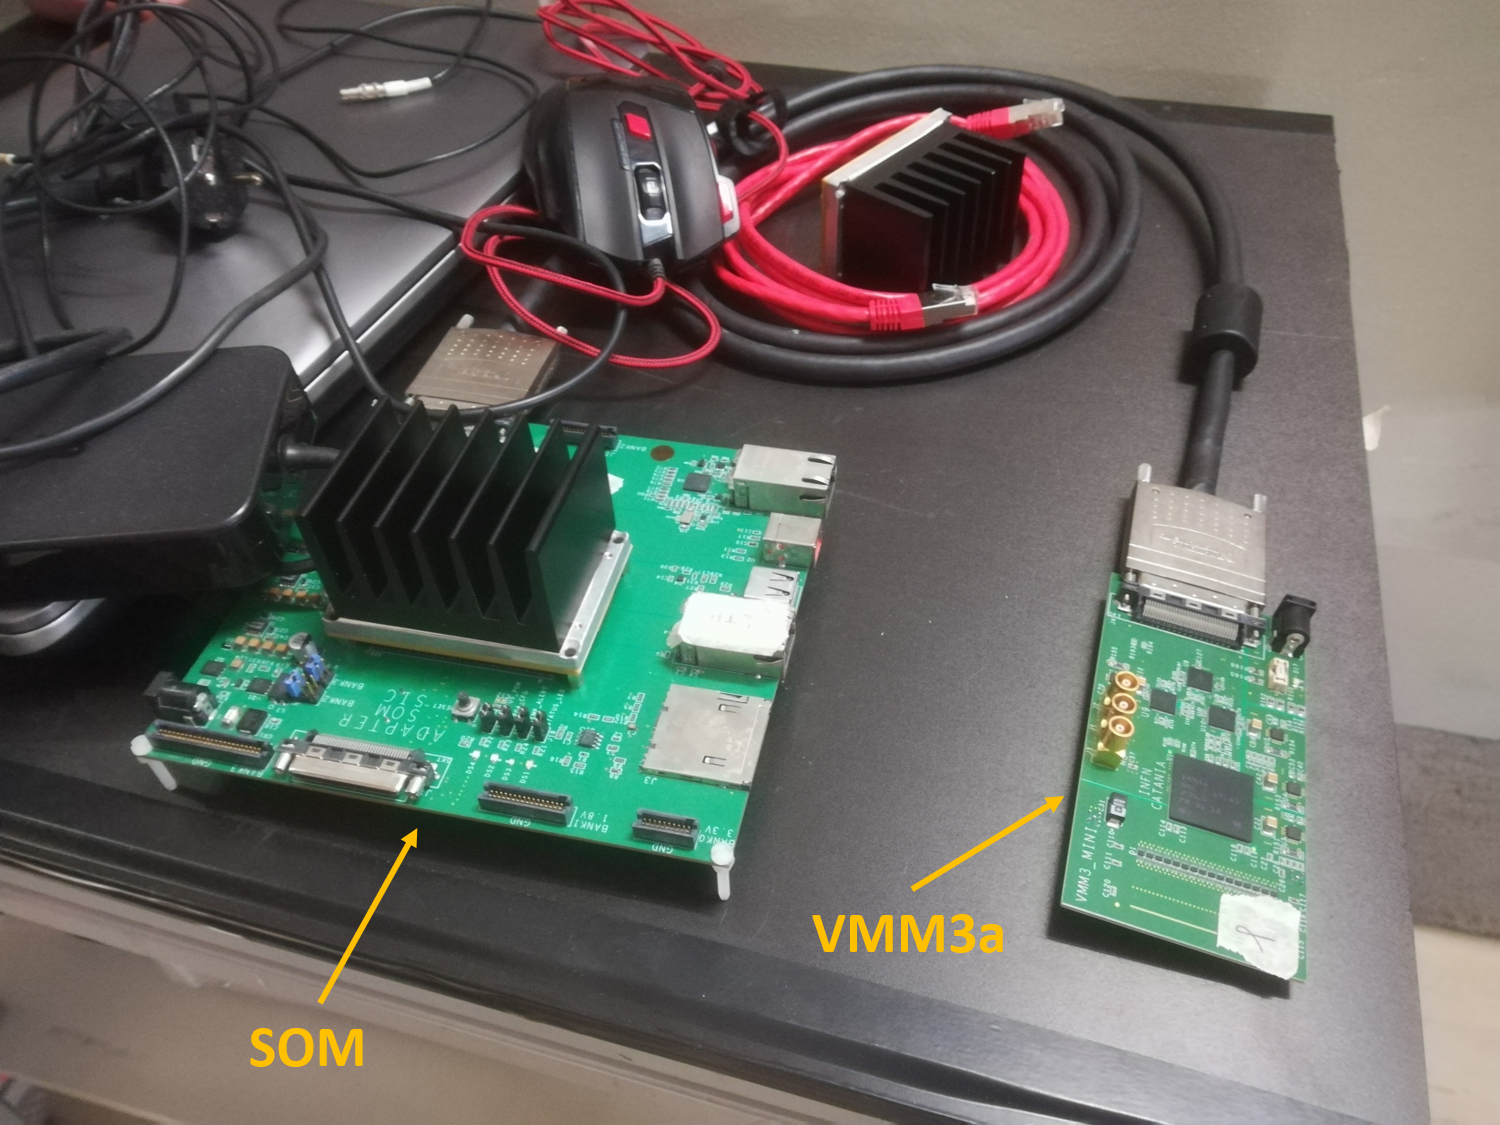
\includegraphics[width=\textwidth, keepaspectratio]{Grafici/vmm3a_som.png}
	\caption{Il chip VMM3a e la scheda SOM utilizzati nel test.} \label{fig:vmm+som}
\end{figure}